\chapter{Highly complex syllable structure: Characteristics, development, and stability}\label{sec:8}
\section{Introduction}\label{sec:8.1}

  In this chapter I consider the findings from the studies in preceding chapters and discuss how they address the broad research questions of the book. In \sectref{sec:8.3} I revisit the first research question, summarizing the evidence for establishing highly complex syllable structure as a linguistic type and discussing how it relates to other holistic language types proposed in the literature. In \sectref{sec:8.4} I return to the second research question and discuss how the various findings inform our understanding of the directionality, tendencies, and mechanisms behind the development of highly complex syllable structure, specifically, and syllable complexity, more generally. In \sectref{sec:8.5} I discuss patterns which suggest that highly complex syllable structure may have long-term stability within languages and language families. Finally, in \sectref{sec:8.6} I suggest some areas for further research.

  Before I move on to those discussions, I present one more brief analysis of the data. A few of the previous analyses dealt with the issue of morphology and syllable complexity. In  \sectref{sec:3.3.6}, the morphological composition of maximal cluster shapes and syllabic consonants was analyzed. It was found that as syllable structure complexity increases, so does the likelihood that the maximal onset and coda patterns of a language display heteromorphemic patterns. Similarly, within most of the syllable structure complexity categories, as syllable structure complexity increases, so does the likelihood that syllabic consonants can be found in grammatical morphemes. While the scope of the book does not allow for a detailed investigation of morphological issues, I present one further analysis in \sectref{sec:8.2} to contribute to our understanding of the role of morphology in the development of highly complex syllable structure and its definition as a language type.

\section{Syllable structure complexity and morphology}\label{sec:8.2}

  In \sectref{sec:1.4.2}, several holistic typologies of language were discussed in which syllable structure complexity is proposed to co-occur with specific morphological properties. Two of the language types proposed by \citet{Skalička1979}, agglutination and introflection, are supposed to have complex consonant clusters. In one of these, agglutination, it is proposed that languages will have a high amount of verbal inflection and more than one inflectional affix per word. However, Skalička’s typology is largely impressionistic and, besides the latter specification, does not provide a method for quantifying the degree of agglutination. \citet{Shosted2006} considers correlations between the potential number of distinct syllable types in a language and inflectional synthesis of the verb. The latter property is defined, following \citet{BickelNichols2005}, as the number of grammatical categories marked on the maximally inflected verb form. Though Shosted’s results were statistically insignificant, the relationship between the two properties was found to be slightly positive among the 32 languages of his sample. These results, along with Skalička’s proposal and the findings in \sectref{sec:3.3.6} regarding morphological patterns of clusters and syllabic consonants, prompt me to investigate the relationship between syllable structure complexity and degree of synthesis in the language sample.

  In morphological typology, synthesis refers to the relative number of morphemes per word in a language. In the morphological typology proposed by \citet{Sapir1921}, the term \textit{synthetic} refers to languages with a few morphemes per word, setting this type apart from \textit{analytic} and \textit{polysynthetic} languages, which have one morpheme per word and many morphemes per word, respectively. Noting the impressionistic nature of these definitions, \citet{Greenberg1954} proposed a quantitative method by which to measure synthesis. This index of synthesis is the average number of morphemes per word in running text. The index does not consider fusion, in which a single morpheme expresses a combination of grammatical meanings (e.g., English 3rd Person Singular Present \textit{-s}). It also does not address some forms of non-concatenative morphology, such as vowel or consonant gradation or subtractive morphology. However, it does capture the relative degree to which affixation and compounding (conflated here) occur in language use. For that reason it is appropriate for the current study. Recall that a prediction made in previous chapters was that large word-marginal consonant clusters may come about when reduction processes affect vowels in unstressed affixes. I expect that this source of large consonant clusters will be reflected in uniformly higher morpheme/word ratios in the Highly Complex category.

  I conducted an analysis to establish the morpheme/word ratios of the languages in the sample. Texts with interlinear glossing were not readily available for all languages, so ultimately this analysis included only 63 of the languages in the sample. The macro-area of Africa is severely underrepresented in this analysis, as texts with interlinear glosses were more difficult to come by for these languages. Only six languages represent Africa, while the other macro-areas are represented by 9-13 languages each.

  It is important to recognize that defining what constitutes a word, either morphosyntactic or phonological, and distinguishing it from a morpheme is not a trivial matter and that the criteria for doing so may be inconsistent among researchers and traditions (\citealt{Haspelmath2011,SchieringEtAl2010}). However, the scope of the current study does not allow for a close examination of these issues. In conducting the morpheme counts, the interlinear glossing in the source was taken at face value. Thus the data may represent a variety of analytical strategies for word and morpheme segmentation. 

  The texts analyzed here represent a variety of genres. Where third-person narratives or traditional stories were available, these were given preference for analysis; however, the texts also include some first-person narratives, dialogues, and formal written prose. Zero morphemes were not counted. On average, the section of text analyzed for each language was about 300 words in length. However, this figure ranges widely from 69 words (for Pech) to 573 words (for Ngarinyin). When fewer than 200 words were analyzed for a language, this typically indicates that no additional texts were available. References for the texts used, as well as raw word and morpheme counts for each language, can be found in Appendix B.

  The means and ranges for morpheme/word ratios for each syllable structure complexity category can be found below.

\begin{table}
\begin{tabularx}{\textwidth}{Qcccc}
\lsptoprule
 & \multicolumn{4}{c}{Syllable structure complexity}\\\cmidrule(lr){2-5}
 Morphemes per word in text & S & MC  & C  & HC\\
                            & \textit{N} = 15 & \textit{N} = 15 & \textit{N} = 17 & \textit{N} = 16\\\midrule
 {Mean} & 1.7 & 1.6 & 1.7 & 2.0\\
 {Range} & 1.0--2.3 & 1.1--2.4 & 1.0--2.8 & 1.1--2.6\\
\lspbottomrule
\end{tabularx}
\caption{\label{tab:8.1}Mean and range values for morpheme/word ratios in running text in languages of sample.}
\end{table}

  The mean morpheme/word value for the entire sample is 1.8. As expected, languages in the Highly Complex category have the highest average number of morphemes per word. Though the range of values observed in this category is similar to the others, the mean shows that more of the languages are distributed towards the high end of the range, indicating a tendency towards, if not a uniformity of, higher morpheme/word ratios in this group. In the 63 languages examined here, there is a statistically significant positive correlation between the morpheme/word ratio and syllable structure complexity. That is, the degree of synthesis generally increases with syllable structure complexity in the sample. This correlation is moderate and statistically significant when syllable structure complexity is measured categorically (\textit{r}(63) = .301, \textit{p} = .02) and weaker when it is measured as a sum of maximal syllable margins (\textit{r}(63) = .261, \textit{p} = .04).

  Though this analysis is very general and glosses over many important issues of morphological analysis, it adds further evidence to the idea that morphology plays an important role in the development of syllable structure complexity. In a sense, this is intuitively understood: many languages with highly complex syllable patterns, including Itelmen, Georgian, Kabardian, Cocopa, and the Salishan languages, have been described as polysynthetic in various descriptions. However, the analysis here establishes a quantitative basis for the relationship and suggests that the presence of a relatively high degree of synthesis is often a prerequisite for the development of highly complex syllable structure. Incidentally, the language in the Highly Complex category with the lowest morpheme/word ratio -- Wutung, with a ratio of 1.1 -- is a language in which Highly Complex syllable patterns are extremely non-prototypical for that group, being restricted to a single tautomorphemic onset with several sonorants, /hmbl/.

  Having further established a role for morphology in patterns of syllable complexity, we now turn to a summary of the evidence for highly complex syllable structure as a linguistic type.

\section{Highly complex syllable structure as a linguistic type}\label{sec:8.3}

  Here I evaluate the results the various studies in this book as they relate to the first central research question \REF{ex:8.1}.

\ea\label{ex:8.1}
   {Do languages with highly complex syllable structure share other phonetic and phonological characteristics such that this group can be classified as a linguistic type?}
\z

  In Chapters 3-7, I presented analyses of the patterns of syllable structure, segmental inventories, suprasegmental properties, vowel reduction, and consonant allophony in a diverse crosslinguistic sample carefully constructed to be equally representative of different degrees of syllable complexity. More often than not, the analyses revealed associations between these features and syllable structure complexity. Below I summarize the strongest patterns which were found to set the Highly Complex category apart from the others in the language sample. Trends found to be statistically significant are marked with an asterisk (*).

\begin{description}
\item[Syllable patterns characteristic of the Highly Complex group (\chapref{sec:3})]
\begin{itemize}[leftmargin=*]
\item[]
\item A large maximal cluster at one syllable margin tends to imply a large cluster at the other margin. {(\sectref{sec:3.3.2})}
\item Obligatory syllable margins (usually onset) frequent in this group.* {(\sectref{sec:3.3.3})}
\item Syllabic consonants most likely to be present in this group.* {(\sectref{sec:3.3.5})}
\item Heteromorphemic patterns in maximal syllable margins most likely in this group.* {(\sectref{sec:3.3.6})}
\item Syllabic consonants more likely to be found in grammatical morphemes in this group. {(\sectref{sec:3.3.6})}
\item Consonant clusters characterized by perceptually salient release, aspiration, variable transitional or intrusive vocalic elements. (\textit{\sectref{sec:3.4.3}})
\end{itemize}

\item[Segmental patterns characteristic of the Highly Complex group (\chapref{sec:4})]

\begin{itemize}[leftmargin=*]
\item[]
\item Largest consonant phoneme inventories (average 26 Cs).* {(\sectref{sec:4.4.1})}
\item Highest average number of articulatory elaborations in consonant phoneme inventories.* (\sectref{sec:6.3.4})
\item Absence of prenasalized consonants* and flap/tap* articulations most likely in this group. {(\sectref{sec:4.4.5})}
\item Presence of palato-alveolar,* uvular,* affricate*, and ejective* articulations most likely in this group. {(\sectref{sec:4.4.4}, \sectref{sec:4.4.5})}
\end{itemize}

\item[Suprasegmental patterns characteristic of the Highly Complex group (\chapref{sec:5})]

\begin{itemize}[leftmargin=*]
\item[]
\item Combination of presence of word stress and absence of tone most likely in this group. {(\sectref{sec:5.4.1})}
\item Stress-conditioned processes affecting consonants least likely to be present in this group. (\sectref{sec:6.3.4})
\item Vowel duration most likely to be phonetic correlate of stress in this group. {(\sectref{sec:5.4.5})}
\end{itemize}

\item[Vowel reduction patterns characteristic of the Highly Complex group (\chapref{sec:6})]

\begin{itemize}[leftmargin=*]
\item[]
\item Vowel reduction most prominent in this group (most likely to be present and most likely to involve two or more distinct processes).* {(\sectref{sec:6.3.1}, \sectref{sec:6.3.2})}
\item Vowel reduction processes least likely to affect high vowels in this group. {(\sectref{sec:6.3.3})}
\item Vowel reduction processes affecting /ə/ occur almost exclusively in this group.* (\sectref{sec:6.3.4})
\item In languages with word stress, word stress conditions the highest average number of vowel reduction processes in this group.* (\sectref{sec:6.3.4})
\item Vowel reduction processes conditioned by word position least common in this group.* (\sectref{sec:6.3.4})
\item Vowel deletion most likely to produce tautosyllabic clusters in this group. (\sectref{sec:6.3.4})
\end{itemize}

\item[Consonant allophony patterns characteristic of the Highly Complex group (\chapref{sec:7})]

\begin{itemize}[leftmargin=*]
\item[]
\item Languages in this group least likely to have allophonic processes resulting in fortition or articulations associated with the Highly Complex category. (\textit{\sectref{sec:7.3.1}})
\item Allophonic processes resulting in palatalization or palato-alveolar articulations least frequent in this group. {(\sectref{sec:7.3.2}, \sectref{sec:7.3.3})}
\end{itemize}

\item[Other morphological patterns characteristic of the Highly Complex group (\chapref{sec:8})]

\begin{itemize}[leftmargin=*]
\item[]
\item Highest degree of synthesis (average morpheme/word ratio) in this group.* {(\sectref{sec:8.2})}
\end{itemize}
\end{description}

  The evidence does indicate that languages on the extreme end of syllable complexity scale share a number of other phonetic and phonological properties in common besides canonical syllable patterns. Most often, these characteristic properties are strong or weak tendencies which set this group apart from languages with simpler syllable structure. However, in a few cases, the properties are near categorical; for instance, vowel reduction patterns affecting only /ə/ were found almost exclusively in the Highly Complex portion of the sample. Moreover, it is often clear from the data that the bundle of features listed above is not a random assortment of phonological properties that just happen to align in this group of languages. In some cases, properties were found to show a gradual linear trend with syllable complexity: e.g., the positive trend with respect to the presence of uvular articulations (\sectref{sec:4.4.5}), or the negative trend with respect to word position in vowel reduction conditioning (\sectref{sec:6.3.4}). In many cases, the trends serve to set the Simple category apart from the three more complex categories: e.g., the absence of phonological asymmetries between stressed and unstressed syllables, or the presence of stress-conditioned consonant allophony. The effect of these interacting patterns is that there are two more or less coherent bundles of phonological tendencies which strongly characterize the languages at either end of the syllable complexity scale. Languages with intermediate syllable patterns (Moderately Complex or Complex) pattern with one or the other of these extremes in many properties, but rarely show different trends altogether, at least not in such a way as to form their own coherent pattern. Additionally, selective statistical testing showed that many of the trends listed above were found to be significant.

  Other evidence pointing to highly complex syllable structure as a linguistic type is in the fact that languages in which these syllable patterns are strong tend to have more of the accompanying phonological features listed above. In \sectref{sec:3.4.2}, I identified two groups of languages in the Highly Complex category based on the size, distribution, combinatorial restrictions, and relative frequency of their Highly Complex syllable patterns. A group of eight genealogically and geographically diverse languages -- Cocopa, Georgian, Itelmen, Polish, Tashlhiyt, Thompson, Tohono O’odham, and Yakima Sahaptin -- were found to have Highly Complex structures as a prevalent pattern in these respects. Another group of six genealogically but less geographically diverse languages -- Alamblak, Bench, Doyayo, Kunjen, Menya, and Wutung -- were found to have Highly Complex structures as a minor pattern according to these criteria. In observing the distribution of other phonological correlates of Highly Complex syllable structure in Chapters 4-6, it was found that these were more strongly associated with languages having Highly Complex structure as a prevalent pattern than those having it as a minor pattern. Languages in which Highly Complex patterns were intermediate tended to behave more like the prevalent group in this respect (see \sectref{sec:4.5.1}, \sectref{sec:5.5.1}, \sectref{sec:6.4.1} for more details).

  As a linguistic type, highly complex syllable structure has properties which are reminiscent of several other language types proposed in holistic (phonological) typologies. The co-occurrence of syllable structure complexity and vowel reduction, especially unstressed vowel reduction, aligns this group of languages with the stress-timed type often discussed in the speech rhythm literature (\citealt{Dauer1983,Auer1993,Schiering2007}). Yet these language types do not completely overlap: in particular, the virtual lack of stress-conditioned consonant allophony and unexpectedly high percentage of fixed stress systems sets languages with highly complex syllable structure apart from prototypical stress-timed languages. Similarly, highly complex syllable structure shares some characteristics in common with the agglutination type proposed by \citet{Skalička1979}, in that syllable complexity co-occurs with a high amount of synthesis (which I liberally take as a proxy for inflection here) and rich consonant systems. Here too the types do not overlap completely, in part because Skalička narrowly defined agglutination so as to approximate an ideal language type. This typology does specify that agglutination is characterized by looser fusion between gramemes and the stem, which would not be reflective of the patterns in the current data, in which large heteromorphemic tautosyllabic consonant clusters often occur. Finally, highly complex syllable structure is particularly aligned with aspects of the consonantal type in the typology proposed by \citet{Isačenko1939/1940}, and with more casual uses of the term in phonological descriptions of languages. Specifically, the co-occurrence of syllable complexity, rich consonant systems, the presence of specific contrasts such as secondary palatalization, and fixed \textit{or} lexically-determined stress in languages with highly complex syllable structure make this type reminiscent of consonantal languages. One major point of departure from this typology is that languages with highly complex syllable structure were found in the current study to be more likely to have syllabic consonants, a feature proposed by Isačenko to co-occur with vocalic languages.

  In sum, the patterns in the data here suggest that highly complex syllable structure is a linguistic type characterized by phonetic, phonological, and morphological patterns which are sometimes categorical but are most often tendencies. Highly complex syllable structure is a holistic language type that shares some features in common with stress-timed languages, agglutination, and consonantal languages, but is also defined by a set of features which are not characteristic of any of those types. In the following section I discuss how the properties of highly complex syllable structure and the other patterns established in this book can be used to address the second research question regarding the historical development of this type.

\section{The development of Highly Complex syllable structure}\label{sec:8.4}

  In this section, I discuss how the findings of the book address the second research question, reproduced below \REF{ex:8.2}.

\ea\label{ex:8.2}
    {How does highly complex syllable structure develop over time?}
\z

  I approach the issue of the development of highly complex syllable structure from several different angles. First, in \sectref{sec:8.4.1} I discuss the issue of assumptions about directionality in syllable structure change, presenting patterns from the current sample which seem to indicate that change more often tends to be in the direction of increased complexity. In \sectref{sec:8.4.2} I discuss how the crosslinguistic patterns established in the preceding chapters might suggest paths of language change associated with the development of this type. In \sectref{sec:8.4.3} I compare the phonological and morphological properties of pairs of related languages differing in their syllable structure complexity in order to determine whether the crosslinguistically established patterns are present at the local level. In \sectref{sec:8.4.4} I discuss a historically attested case of syllable structure change and how it relates to the findings in this book. In \sectref{sec:8.4.5} I discuss issues of language contact and the transfer of prosodic properties from one language to another as one potential source for the development of highly complex syllable structure. Finally, in \sectref{sec:8.4.6} I present some ideas for how such processes might get started in a language.

\subsection{Directionality of syllable structure change}\label{sec:8.4.1}

  Up until this point, it has been assumed when discussing the phonetic and phonological correlates of syllable structure complexity that the findings might point to how highly complex syllable structure develops out of simpler syllable patterns. In many cases I have referred to the four-category syllable structure complexity scale used in this study as corresponding to a diachronic cline. This assumption is, in part, supported by documented evidence of such a cline: for example, we can be certain from historical records that the present syllable patterns of Lezgian, which have been mentioned several times previously, arose out of simpler patterns. However, since the focus has been on processes which create syllable complexity, the opposite scenario, in which the phonetic and phonological correlates might be interpreted to reflect instead how simple syllable structure develops out of more complex patterns, has been largely neglected.

  There is ample evidence within the language sample for syllable structure change going in the direction of increased complexity. The analysis of outcomes of vowel deletion in \sectref{sec:6.3.5} provides many such examples. Eight languages were found to have vowel deletion resulting in non-canonical simple codas: in Sumi Naga, Tukang Besi, Lunda, and Camsá, such processes create codas in languages that otherwise do not have them; and in Saaroa, Atong, Cocama-Cocamilla, and Lakota, the processes add new consonants to the inventory of simple codas in the language. In a similar case, while word-internal codas already occur in Kambaata, a process of vowel devoicing and deletion has started to produce these codas word-finally. This has not changed the canonical syllable patterns of the language, but it is having an effect on the phonological shape of words, which previously ended only in vowels. Additionally, eight languages have vowel deletion processes resulting in non-canonical tautosyllabic clusters: in Southern Grebo, Sumi Naga, Choctaw, and Karok, these processes create clusters in syllable margins which are otherwise simple; in Eastern Khanty and Nuu-chah-nulth, these processes create larger clusters than what the language canonically has; and in Albanian and Qawasqar, these processes create clusters which are the same size as canonical clusters but of non-canonical shapes.

  Apart from the cases above involving synchronic vowel deletion, there are at least eight additional languages in the sample for which historical, comparative, and other evidence points to syllable structure recently having become more complex. Several of these were mentioned in \sectref{sec:3.2.3} in the discussion of languages whose patterns fell near the edges of the syllable structure complexity categories as defined in this study. Cavineña and Ute are classified as having Simple syllable structure, but both have canonical simple codas which have recently arisen as a result of vowel deletion. In some languages, speech style and sociolinguistic variation suggest that syllable structure has recently become more complex. In Pech, onset clusters /pɾ, tɾ, kɾ, bɾ/ appear to be a recent development as a result of syncope of historical or underlying vowels, as the vowels may “reappear” in slow speech \citep[20]{Holt1999}. Similarly, in Oksapmin, biconsonantal onset clusters are realized with an intervening schwa for some older speakers, but are produced as clusters by most younger speakers \citep[65-67]{Loughnane2009}. Bruce notes that close transition in consonant clusters in Alamblak corresponds to /ɨ/ in related language Sumariup (\citeyear[69--70]{Bruce1984}). He takes this as likely evidence of recent vowel deletion in Alamblak, since the remaining occurrences of /ɨ/ in the language are weak with respect to stress placement and susceptible to elision. Writing conventions can also point to the directionality of the change. As mentioned in \sectref{sec:3.4.3}, changing writing conventions in Menya may suggest that the clusters in that language are a product of recent vowel reduction and deletion (\citealt{Whitehead2004}: 9, 226). In Lezgian, the process of high vowel syncope which has recently made syllable patterns more complex is well-documented by orthographic evidence \citep[36-8]{Haspelmath1993}. Finally, in Tzeltal, syllable patterns have recently become more complex as a result of loanwords becoming nativized. The largest native onsets in the language are of the form /s ʃ h/ + C\textsubscript{2}, with the initial consonant corresponding to a prefix. Kaufman reports that these prefixes may now be attached to Spanish loanwords with initial consonant clusters, resulting in triconsonantal onsets \citep[14]{Kaufman1971}.

  It is far rarer to find clear cases of ongoing simplification of native canonical syllable structure patterns in the language sample. Variable processes of cluster-simplifying vowel epenthesis and consonant deletion were not systematically collected for all languages of the sample; however, they were noted wherever observed.\footnote{{Note that cases of (morpho)phonological epenthesis are not considered in this discussion. Recall from the discussion of methods in \sectref{sec:3.2.1} that processes of vowel epenthesis which were reported to be invariant were considered to be part of the canonical syllable pattern of the language.}} There are four languages in the sample for which the canonical syllable structure seems to be unambiguously undergoing simplification. The case of Towa was discussed in \sectref{sec:3.2.3}. In this language, which has canonical simple codas, processes of coda deletion operate in all environments except for utterance-finally \citep[22-4]{Yumitani1998}. The resulting extremely low frequency of phonetic codas is what justified the inclusion of this language in the Simple category. In Passamaquoddy-Maliseet, apostrophes are now used in the practical orthography to represent consonants which were once pronounced but are now absent from clusters (e.g., \textit{‘tomake\'{} yˑu} is the modern spelling of what was once \textit{ktomake\'{} yˑu} ‘s/he is poor,’ \citealt{Leavitt1996}: 16). It is known from historical transcriptions and the pronunciation of older speakers that these were originally clusters and have recently undergone simplification. In Chipaya, historical records indicate that triconsonantal onsets used to occur as a result of the affixation of personal prefix \textit{x-}. At present such forms are reported to be obsolete and completely unproductive, though speakers do passively accept them (citealt{Cerrón-Palomino2006}: 66). In Atong, some non-initial syllables vary between C+/əɾ/ and C+/ɾ/ shapes, the latter being the only complex onsets attested in the language. While \citet[30--32]{VanBreugel2008} analyzes this as a process of vowel reduction, comparative evidence from the family suggests that the C+/ɾ/ clusters are original, with some having been historically resolved through consonant deletion and others variably resolved synchronically through schwa insertion.

  There are also several ambiguous cases of active syllable structure simplification in the language sample. In the Vietnam dialect of Kim Mun, Clark observes central vowel insertion between the consonants in one of the biconsonantal onset patterns, /kl/ \citep[127]{Clark2008}. However, this report is based on one token in the speech of one informant, and it is not clear whether this may be a frequent variant of the cluster. In Qawasqar, triconsonantal onsets, including /qsq/ and /qst/, are reported to be unstable in rapid speech: e.g., \textit{qsqaɾ} > \textit{sqaɾ}, ‘urine’ \citep[393]{Clairis1985}. However, in this language rapid speech may also produce clusters through vowel deletion -- e.g. \textit{seqwe} > \textit{sqwe} ‘future marker’ -- so it is unclear whether syllable structure complexity is changing significantly in either direction in this language. Finally, as discussed in \sectref{sec:3.2.3}, Yine also presents an ambiguous case of syllable structure change. \citet[24]{Matteson1965} states that the very low frequency of triconsonantal onsets had decreased in comparison to a count made a decade previously. However, \citet[27]{Hanson2010}, writing nearly half a century later, writes that “words beginning with three consonants in a sequence are very common”.

  Taking all of the above patterns into account, there are 24 languages in the sample in which synchronic, historical, or comparative evidence suggests that canonical syllable structure has become or is becoming more complex. By comparison, there are four languages in which similar evidence strongly suggests that canonical syllable patterns have become or are becoming simpler. For one language (Vietnam Kim Mun), a very weak case could be made for simplification. Finally, Qawasqar and Yine present ambiguous cases in which canonical syllable structure change does not show a preference for directionality, or there are conflicting reports regarding this phenomenon.

  Interestingly, one of the strong cases for ongoing syllable structure simplification is from an obsolescing language, Passamaquoddy-Maliseet. This outcome is consistent with observations by \citet{Romaine2010} and \citet{Cook1989} regarding the effect of obsolescence on phonological structure. However, it should be noted that several obsolescing languages, including Cocama-Cocamilla, Choctaw, and Karok, have processes of vowel reduction which make syllable patterns more complex.

  There are many historically documented cases of syllable structure simplification. Historical and modern varieties of English provide a number of such examples: e.g., simplification of /kn/ and /ɡn/ onsets in Middle English \citep{Minkova2003}, coda deletion and simplification in African American Vernacular English \citep{Rickford1999}, and coda simplification and debuccalization in Singapore English \citep{Deterding2007}. Invariant (morpho)phonological vowel epenthesis having the effect of preserving canonical syllable patterns is commonly reported in the language sample examined here; perhaps some of these are the result of historical phonetic processes which have become phonologized. However, as a gradient, phonetically motivated process, simplification of syllable structure seems to be reported more rarely than an increase in syllable structure complexity as a result of vowel reduction. That is, the reported phonetic patterns in the language sample suggest that syllable structure change is more often in the direction of increased complexity. This is a puzzling result when the crosslinguistic distribution of syllable complexity is considered. If reported phonetic processes are indicative of a uniform trend towards complex syllable structure, we would perhaps expect the global proportions of languages with Complex and Highly Complex syllable patterns to be much higher than they are. I do not discount that the distribution of phonetic processes discussed above could reflect common biases in phonological analysis, or perhaps even more rapid phonologization of vowel epenthesis and consonant deletion patterns as compared to vowel reduction and deletion patterns, for whatever reason. Perhaps ongoing research on listener/researcher bias in identifying syllable patterns (e.g., \citealt{KwonEtAl2017}) could shed some light on this paradox.

\subsection{Clues from the crosslinguistic patterns}\label{sec:8.4.2}

  We know from historically documented processes of syllable structure change in specific languages that unstressed vowel deletion is a common source of the consonant clusters associated with highly complex syllable structure. Snapshots of ‘before’ and ‘after’ states of syllable patterns in a language are useful because they illustrate the direct and dramatic effect of unstressed vowel deletion on syllable structure. However, such reports might overlook the relationship between these processes and other parts of the phonology and grammar. If the reductive patterns which eventually manifest as vowel deletion have a long history in a language, effects that they have long before vowel deletion becomes prevalent may not be recognized as directly related to the process of syllable structure change. Examination of the crosslinguistic trends may reveal these subtle patterns and allow us to ‘fill in’ other crosslinguistically common steps in the process which might not otherwise be apparent when looking at specific case studies. Trends in syllable patterns, segmental inventories, suprasegmental properties, and processes of vowel reduction and consonant allophony established in the prior chapters suggest some potential links in the chain of developments leading to the emergence of highly complex syllable structure.

  An interesting finding in the analysis of syllable structure in \sectref{sec:3.3.2} was that large maximal clusters in one syllable margin tend to imply similarly large maximal clusters in the other syllable margin. As mentioned in that analysis, this is not an expected distribution if we consider onsets and codas to be independent structures. From a diachronic point of view, this suggests that complex onset and coda patterns may not be independent in terms of their development, especially in situations of extreme vowel reduction and loss. This relates to the findings regarding the morphological complexity of highly complex clusters (\sectref{sec:3.3.6}) and the higher degrees of synthesis observed in these languages (\sectref{sec:8.2}). Assuming morphologically or lexically conditioned stress, in a language with a high degree of synthesis and both prefixation and suffixation, we would expect processes of unstressed vowel deletion to create large heteromorphemic consonant clusters at both word edges. Also related to these issues are the findings that syllabic consonants are more frequently found in the Highly Complex portion of the sample, and that these are most frequently found to belong or correspond to grammatical morphemes in that group. Such patterns may reflect similar sources of unstressed vowel reduction in affixes, though perhaps with different temporal effects on articulation.

  The analysis of segmental patterns in \chapref{sec:4} similarly revealed that languages in the Highly Complex category are more likely to have specific consonant articulations than other languages in the sample. In particular, palato-alveolar, uvular, ejective, and affricate articulations were strongly associated with this category. A survey of historical and synchronic processes known to produce these articulations revealed that these tend to come about through processes of assimilation and fortition, which often correspond to the temporal overlap of consonant and vowel (or glottal) articulations, or strengthening of gestures in certain domain or vocalic environments. The tendency of languages in the Highly Complex category to have such sounds suggests that such processes were once prevalent enough in the languages’ histories to phonologize into segmental patterns. Further, the presence of such segments in a language becomes more likely with increasing syllable structure complexity, which suggests that these processes may be interconnected in some way with the development of complex syllable patterns.

  The analysis of suprasegmental patterns in \chapref{sec:5} yielded some unexpected results, in that the Highly Complex category was not found to be strongly associated with lexically- or morphologically- conditioned word stress. Additionally, languages with Highly Complex syllable structure were not found to be substantially more likely to have unstressed vowel reduction than languages in the Moderately Complex or Complex categories. The latter result was elucidated in the study of vowel reduction in \chapref{sec:6}. There it was found that in languages with unstressed vowel reduction, the average number of distinct processes of that kind increased with syllable complexity. This suggests a sort of ‘snowball effect’ in which vowel reduction patterns conditioned by stress may gradually become more prevalent in a language even as syllable patterns are affected in their wake. What causes this increasing reductive tendency is not entirely clear. It was expected that such extreme effects of stress would be more likely in languages with morphologically- or lexically-conditioned (unpredictable) stress, as previously found in the literature (\citealt{BybeeEtAl1998,Schiering2007}). However, most of the stress systems in the Highly Complex group are not unpredictable. Of those languages which do have unpredictable stress, most have an average number of vowel reduction processes for that group (2 processes). Meanwhile, some languages with fixed or weight-dependent stress have a higher than average number of vowel reduction patterns (Tohono O’odham with 7, Kabardian with 4, Yine with 3; among others). 

  One diachronic account for this unexpected mismatch between the vowel reduction patterns and the stress patterns could be that languages with Highly Complex syllable structure are likely to have had unpredictable stress systems at an earlier point in their histories. In such a scenario, a language with relatively simple syllable structure and lexically- or morphologically-determined stress patterns and a high degree of synthesis develops a pattern of unstressed vowel reduction. As vowels are reduced and deleted, stress shifts accordingly with respect to word edges. Say in such a scenario that stress is stem-initial and the language has phonologically short, unstressed grammatical prefixes. If vowel reduction deleted all vowels in prefixes in such a language, it could eventually have the effect of causing the stress system to become a fixed initial system rather than an unpredictable system. Such processes, if crosslinguistically common, could account for the unexpectedly high rate of fixed stress systems in the Highly Complex group.

  There are a few other crosslinguistic findings that may relate to the diachronic development of syllable structure complexity. In \chapref{sec:6} it was found that deletion of /ə/ was a common process type in the Highly Complex category. In fact, though phonemic /ə/ could be found in languages from all categories of syllable structure complexity, this sound was specifically targeted for further reduction almost exclusively in languages in the Highly Complex category. Since [ə] is often the outcome of vowel reduction, processes reducing or deleting /ə/ may be indicative of a long history of vowel reduction in a language.

  Finally, the analyses in \chapref{sec:7} sought in part to determine the distribution of allophonic processes producing articulations associated with the Highly Complex category, as well as other specific processes of consonant assimilation to vowels and fortition. It was found that processes producing palato-alveolars, affricates, palatalization, and increased constriction, specifically, were more prevalent in languages with Simple syllable structure. Further, stress conditions more such processes in languages of the Simple category than in others. When this trend is plotted against the trend for stress-conditioned vowel reduction, the resulting pattern indicates that as syllable structure complexity increases, stress decreasingly affects consonants and increasingly affects vowels. If the syllable structure complexity scale is taken to be a diachronic cline, what this suggests is that, during the development of syllable structure complexity, stress affects consonants first and vowels later. Though the results in \chapref{sec:7} did not paint so straightforward a picture, what this suggests in terms of syllable complexity and segmental inventories is that consonant articulations associated with the Highly Complex group may develop before the syllable patterns associated with these languages.

  As mentioned in previous chapters, there is always the risk when conducting typological studies that strong crosslinguistic trends may be an epiphenomenon emerging from several distinct smaller-scale patterns. Many of the analyses in this book have shown that is not the case, as the patterns can be found in diverse groups of languages. However, it is important to see if the diachronic paths which have been inferred from the crosslinguistic trends are plausible at a local level before positing them to be common paths of syllable structure change. In the following section I conduct such a study.

\subsection{Comparisons of related pairs of languages in sample}\label{sec:8.4.3}

  Recall in \sectref{sec:2.1.3} that the language sample was constructed so as to include pairs of related languages with differing degrees of syllable structure complexity. Here we compare these pairs to see if the crosslinguistic associations between syllable structure complexity and phonological and morphological patterns hold at the local level, in which case the diachronic paths discussed above may be more plausible. Where relevant, I also mention historical and comparative evidence that may further shed light on the mechanisms behind the divergent patterns.

\subsubsection{{Uto-Aztecan:} {Ute} {and} {Tohono} {O’odham}}\label{sec:8.4.3.1}

  Ute and Tohono O’odham both belong to the Uto-Aztecan family of languages, a family with large geographic spread in the western region of the USA and Mexico. Ute is a member of the Numic branch of the Northern division of the family, which also includes Shoshone, Northern Paiute, and Chemehuevi. At time of contact with Spanish and Anglo settlers, it was indigenous to the mountains of western Colorado and eastern Utah \citep{Givón2011}. Tohono O’odham is a member of the Tepiman branch of the Southern division. This branch includes its close relative Pima as well as the Tepehuan languages of northern Mexico. It is spoken in southern Arizona and northern Sonora \citep{Zepeda1983}.

  Ute has been classified in the Simple category in the current language sample, though its syllable patterns are technically Moderately Complex (see discussion in \sectref{sec:3.2.3}). Tohono O’odham has Highly Complex syllable structure as a prevalent pattern. A summary of the phonological properties of these languages, as they relate to the findings of the previous chapters, can be found in \tabref{tab:8.2}.

\begin{table}
\small
\begin{tabularx}{\textwidth}{III}
\lsptoprule
 & {Ute} & {Tohono O’odham}\\
 \midrule
 {Syllable patterns} & Simple & Highly Complex (prevalent)\\
 \tablevspace 
 {Maximal syllable margins} & Onset: 1; Coda: 1 & Onset: 4; Coda: 4\\
 \tablevspace 
 {Syllabic consonants} & -- & obstruents\\
 \tablevspace 
 {C phoneme inventory} & /p t k ʔ t͡ʃ β s ɣ m n ɾ w j/ & /p b t̪ d̪ ɖ k ɡ ʔ t͡ʃ d͡ʒ s̪ ʂ h m n̪ ɲ ŋ ɭ β ̞ j/\\
 \tablevspace 
 {N C phonemes} & 13 & 20\\
 \tablevspace 
 {Articulations/contrasts associated with {Simple}} {category} & {Flap/tap} & {Flap/tap}\\
 \tablevspace 
 {Articulations/contrasts associated with {Highly Complex}} {category} & { {Palato-alveolar}} 
 
 Affricate& { {Palato-alveolar}}
 
 Affricate\\
 \tablevspace 
 {Word stress present?} & {Yes} & {Yes}\\
 \tablevspace 
 {Stress placement} & {Fixed} & {Fixed}\\
 \tablevspace 
 {N V reduction processes} & {3} & {7}\\
 \tablevspace 
 {Vs affected by reduction}  & {all} & {all, high, short}\\
 \tablevspace 
 {V reduction environments} & {Consonant, Stress, Word} & {Consonant, Stress, Word, Phrase}\\
 \tablevspace 
 {V reduction outcomes} & {Devoicing} & {Devoicing, Quality, Deletion}\\
 \tablevspace 
 {C allophony resulting in S articulations, lenition/sonorization} & {{Flapping}}\newline {{Obstruent voicing}}\newline  {Spirantization} & {--}\\
\tablevspace 
 {{C allophony resulting in HC articulations,} }\newline  {C-to-V assimilation, fortition} & {{Uvular}}\newline { {Labialization}}\newline  {Palatalization} & {Glide strengthening}\\
\lspbottomrule
\end{tabularx}
\caption{\label{tab:8.2}Comparison of phonological properties of Ute and Tohono O’odham.}
\end{table}

  This segmental patterns of this pair of Uto-Aztecan languages largely conforms to the crosslinguistic patterns established in previous chapters for Simple and Highly Complex syllable structure. Tohono O’odham has syllabic obstruents, while Ute has no syllabic consonants at all. The consonant phoneme inventory of Tohono O’odham is larger than Ute’s by seven consonants. However, both languages have consonant articulations which are associated with both the Simple and Highly Complex categories: both have flap/tap, palato-alveolar, and affricate articulations.

  The suprasegmental and allophonic patterns of Ute and Tohono O’odham are also somewhat in line with the predictions. Both languages have word stress and vowel reduction, but the number of distinct reductive patterns in Tohono O’odham is much greater. While both languages have both domain- and stress-conditioned vowel reduction, the number and extremity in outcomes is greater for Tohono O’odham, and processes also target short and high vowels in this language. Ute has a wide variety of allophonic processes affecting consonants. These include assimilation of consonants to vowels -- including a process that produces uvulars, a Highly Complex-associated articulation -- as well as processes of lenition and sonorization. Of the synchronic processes considered here, Tohono O’odham only has glide strengthening. Interestingly, glide strengthening has been proposed as a historical source for the voiced stop series in Tepiman languages. In fact, this typologically rare sound change is one of the phonological features which sets Tepiman apart from the other branches of Uto-Aztecan (\citealt{ShaulHill1998}: 379).

  Finally, the morphological patterns of the two languages show mixed results. Ute has a much higher morpheme/word ratio than Tohono O’odham: 2.3 as compared to 1.4. This does not follow the general crosslinguistic pattern. However, more in line with predictions, in Tohono O’odham all of the maximal syllable onset and coda patterns are heteromorphemic, and syllabic obstruents always correspond to grammatical particles (determiners and conjunctives, specifically).

  Of the two languages examined here, Ute has syllable patterns which are more typical of general Uto-Aztecan patterns. Of the seven Uto-Aztecan languages included in the survey by \citet{Maddieson2013a}, four languages have Moderately Complex syllable structure, two Complex, and the remaining language is Tohono O’odham. This suggests that the Tohono O’odham syllable patterns are a novel and perhaps relatively recent development in the family. Indeed, variable and invariable processes of final vowel deletion are noted in most Tepiman languages, suggesting a long history of vowel reduction affecting phonotactics in this branch of the family (\citealt{ShaulHill1998}: 384-5). However, even among the Tepiman languages, the syllable structure of Tohono O’odham is unusually complex (cf. canonical (C)V(C) patterns in Pima Bajo,  \citealt{EstradaFernández2014}: 40). Comparing the consonant allophony processes of Ute against the consonant phoneme inventory of Tohono O’odham, and the details of vowel reduction processes in the former versus the latter, it does seem plausible that the phonological patterns of Tohono O’odham evolved from a system that once looked more like Ute.

  Interestingly, the Tepiman branch of Uto-Aztecan has likely had a long history of contact with the Yuman language family, to which Cocopa (Highly Complex) belongs. \citet{ShaulHill1998} argue that phonological evidence, grammatical convergence, and borrowings suggest heavy contact between Proto-Tepiman and Proto-River-Yuman starting during the Hohokam period in the first millennium C.E.

\subsubsection{{Arawakan:} {Apurinã} {and} {Yine}}\label{sec:8.4.3.2}

  Apurinã and Yine both belong to the Arawakan family of languages, a large language family with wide geographical spread throughout Central America and the northern half of South America. Apurinã and Yine both belong to the small Purus branch of Arawakan, a subclassification within the larger Southern Maipuran branch. Apurinã is said to be Yine’s closest linguistic relative \citep{Facundes2002}. Apurinã is spoken along the tributaries of the Purús River in the southern part of Amazonas state in Brazil, while Yine is spoken in the Madre de Dios region of Peru \citep{Aikhenvald1999}.

  Apurinã has Simple syllable structure, while Yine has been classified as having Highly Complex syllable structure as an intermediate pattern (see discussion in \sectref{sec:3.2.3} about complications for classifying syllable patterns in Yine). A summary of the phonological properties of these languages can be found in \tabref{tab:8.3}.

\begin{table}
\small
\begin{tabularx}{\textwidth}{III}
\lsptoprule
 & {Apurinã} & {Yine}\\
 \midrule 
 {Syllable patterns} & Simple & Highly Complex (intermediate)\\
 \tablevspace
 {Maximal syllable margins} & Onset: 1; Coda: 0 & Onset: 3; Coda: 0\\
 \tablevspace
 {Syllabic consonants} & -- & (conflicting reports)\\
 \tablevspace
 {C phoneme inventory} & /p t k t͡s t͡ʃ s ʃ h m n ɲ ɾ j ɰ/ & /p t c k t͡s t͡ʃ s ʃ ç ɦ m n l ɾ w j/\\
 \tablevspace
 {N C phonemes} & 14 & 16\\
 \tablevspace
 {Articulations/contrasts associated with {Simple}} {category} & {Flap/tap} & {Flap/tap}\\
 \tablevspace
 {Articulations/contrasts associated with {Highly Complex}} {category} & { {Palato-alveolar}}\newline  {Affricate} & { {Palato-alveolar}}\newline  {Affricate}\\
 \tablevspace
 {Word stress present?} & {Yes} & {Yes}\\
 \tablevspace
 {Stress placement} & {Weight-sensitive} & {Fixed}\\
 \tablevspace
 {N V reduction processes} & {1} & {3}\\
 \tablevspace
 {Vs affected by reduction}  & {all} & {all, /a/}\\
 \tablevspace
 {V reduction environments} & {Stress, Word} & {Stress, Word, Phrase/Utterance}\\
 \tablevspace
 {V reduction outcomes} & {Devoicing} & {Devoicing, Quality}\\
 \tablevspace
 {C allophony resulting in S articulations, lenition/sonorization} & {Obstruent voicing} & { {Flapping}}\newline  {Obstruent voicing}\\
 \tablevspace
 {{C allophony resulting in HC articulations,} }\newline  {C-to-V assimilation, fortition} & {Palatalization} & { {Affricate}}\newline  {Increased constriction}\\
\lspbottomrule
\end{tabularx}
\caption{\label{tab:8.3}Comparison of phonological properties of Apurinã and Yine.}
\end{table}

  As mentioned in \sectref{sec:3.3.5}, there are conflicting reports as to whether Yine has syllabic consonants. \citet{Matteson1965} describes the syllable template as having complex onsets, but also describes the consonants which do not directly precede the nucleus as being syllabic allophones of the consonants. In \chapref{sec:3} I took the onset cluster analysis. In any case, it does not affect the analysis of the language as having Highly Complex syllable structure.

  The segmental patterns of Apurinã and Yine show mixed results with respect to the predicted patterns. The consonant phoneme inventory of Yine is larger than that of Apurinã by two consonants, as predicted. Both languages have two articulations associated with the Highly Complex category (palato-alveolar and affricate) and one articulation associated with the Simple category (flap/tap). Comparing the inventories we see that Yine has one more obstruent in the general palatal region than Apurinã. This latter pattern is in line with the crosslinguistic pattern observed in \sectref{sec:4.4.4}.

  In terms of suprasegmentals and allophonic patterns, we find that both languages have word stress and vowel reduction. Yine has more distinct vowel reduction patterns than Apurinã, as predicted. Yine also has reduction in quality outcomes as predicted. However, both languages have vowel reduction, and specifically devoicing, in stress and domain contexts. As for consonant allophony, the pattern is the opposite of what is predicted: Yine has more such processes, including those of the assimilation/fortition types.

  The morpheme/word ratio is 2.1 for both Apurinã and Yine, which is unsurprising given how closely the languages are related. In Yine, maximal onset clusters are heteromorphemic, though biconsonantal onsets may show tautomorphemic or heteromorphemic patterns. If the syllabic consonant analysis is taken, syllabic consonants would occur in both grammatical and lexical morphemes.

  Of the two languages compared here, the syllable patterns of Apurinã are more closely aligned with the general patterns of the Arawakan family. Of the six Arawakan languages included in the survey in \citet{Maddieson2013a}, five of them have Moderately Complex syllable structure, none have Complex syllable structure, and the other language is Apurinã. Since Yine and Apurinã are very closely related, this suggests that the highly complex patterns of Yine may have developed relatively recently in history. Comparing cognate forms in Apurinã and Yine given in \citet[88-9]{Facundes2002}, missing vowels in the Yine forms correspond to /i e ɨ a o/ in the Apurinã forms, suggesting that the historical vowel deletion processes responsible for creating consonant clusters in Yine were quite general.

\subsubsection{{Atlantic-Congo:} {Yoruba} {and} {Lunda}}\label{sec:8.4.3.4}

  Yoruba and Lunda both belong to the Atlantic-Congo family of languages, a huge language family which is spread throughout most of sub-Saharan Africa. There are several taxonomic systems by which the languages in this family are classified and related to one another, some of them conflicting. In my discussion here, I follow the classification system proposed by \citet{Williamson1989}. In this classification, both Yoruba and Lunda belong to different genera within the Benue-Congo branch of the Volta-Congo subfamily. Yoruba, native to Nigeria and now a major language of West Africa, belongs to the Defoid genus. Lunda belongs to the large Bantoid genus, and is spoken in northwestern Zambia \citep{Kawasha2003}.

  Yoruba has Simple syllable structure and Lunda has Complex syllable structure. A summary of the phonological properties of these languages can be found in \tabref{tab:8.4}.

\begin{table}
\small
\begin{tabularx}{\textwidth}{III}
\lsptoprule
 & {Yoruba} & {Lunda}\\
 \midrule 
 {Syllable patterns} & Simple & Complex\\
 \tablevspace
 {Maximal syllable margins} & Onset: 1; Coda: 0 & Onset: 3; Coda: 0\\
 \tablevspace
 {Syllabic consonants} & nasals & --\\
 \tablevspace
 {C phoneme inventory} & /b t d ɟ k ɡ k͡p ɡ͡b f s ʃ h m l ɾ j w/ & /p b t d k ɡ t͡ʃ d͡ʒ f v s z ʃ ʒ h m n ɲ ŋ l w j/\\
 \tablevspace
 {N C phonemes} & 17 & 22\\
 \tablevspace
 {Articulations/contrasts associated with {Simple}} {category} & {Flap/tap} & {--}\\
 \tablevspace
 {Articulations/contrasts associated with {Highly Complex}} {category} & {Palato-alveolar} & { {Affricate}}\newline  {Palato-alveolar}\\
 \tablevspace
 {Word stress present?} & {No} & {(Not reported)}\\
 \tablevspace
 {Stress placement} & {--} & {--}\\
 \tablevspace
 {N V reduction processes} & {--} & {1}\\
 \tablevspace
 {Vs affected by reduction}  & {--} & {/i/}\\
 \tablevspace
 {V reduction environments} & {--} & {Consonant, Word}\\
 \tablevspace
 {V reduction outcomes} & {--} & {Deletion}\\
 \tablevspace
 {C allophony resulting in S articulations, lenition/sonorization} & {--} & {--}\\
 \tablevspace
{ {C allophony resulting in HC articulations,} }\newline  {C-to-V assimilation, fortition} & {--} & {--}\\
\lspbottomrule
\end{tabularx}
\caption{\label{tab:8.4}Comparison of phonological properties of Yoruba and Lunda.}
\end{table}

  The segmental patterns of Yoruba and Lunda largely follow the predictions. Lunda does has a consonant phoneme inventory which is larger than Yoruba’s by five consonants. Both languages have palato-alveolar consonants (typically associated with the Highly Complex category), but Yoruba additionally has a flap and Lunda additionally has affricates, in line with the established crosslinguistic generalizations.

  There is not much to compare in terms of the suprasegmental properties and allophonic patterns of the two languages. Yoruba does not have stress and it is not reported whether Lunda has stress in the reference consulted. Lunda has one vowel reduction process with an extreme outcome of vowel deletion. Neither language is reported to have any of the allophonic consonant processes considered here.

  Morpheme/word ratios could not be calculated for Yoruba or Lunda due to lack of available texts. However, the other morphological patterns show mixed results. Triconsonantal onset clusters in Lunda are always morphologically complex, occurring when a class prefix is affixed to a noun, among other possibilities \citep[23-24]{Kawasha2003}. While Lunda does not have any syllabic consonants, Yoruba has syllabic nasals which always correspond to grammatical morphemes.

  Neither of the two languages have syllable patterns typical of Atlantic-Congo, the languages of which show a range of patterns but tend most often to be Moderately Complex \citep{Maddieson2013a}. In Lunda, it is clear that the development of syllable complexity is at least partly to the morphology of the language: the largest clusters in the language occur only in heteromorphemic contexts.

\subsubsection{{Indo-European:} {Darai} {and} {Albanian}}\label{sec:8.4.3.5}

  Darai and Albanian both belong to the Indo-European family of languages, a large family which is spread throughout much of Eurasia. Darai is a member of the large Indo-Iranian genus of the family which is located in South Asia. It is spoken along the Narayani and Madi Rivers in Nepal \citep{Dhakal2012}. Albanian constitutes its own branch within Indo-European. The Tosk dialect included in this study is spoken south of the Shkumbin River in Albania and northern Greece, and corresponds closely to the standard form of the language. The time depth of separation between these languages is estimated to be at least 4000 years \citep[146]{Garrett2006}.

  Darai has Moderately Complex syllable structure, while Albanian has Highly Complex syllable structure as an intermediate pattern in the language. A summary of the phonological properties of these languages can be found in \tabref{tab:8.6}.

\begin{table}
\small
\begin{tabularx}{\textwidth}{III}
\lsptoprule
 & {Darai} & {Albanian}\\
 {Syllable patterns} & Moderately Complex & Highly Complex\newline (intermediate)\\
 \midrule 
 {Maximal syllable margins} & Onset: 2; Coda: 1 & Onset: 4; Coda: 3\\
 \tablevspace
 {Syllabic consonants} & -- & --\\
 \tablevspace
 {C phoneme inventory} & /p b t̪ d̪ ʈ ɖ k ɡ pʰ bʰ t̪ʰ d̪ʰ ʈʰ ɖʰ kʰ ɡʰ t͡s d͡z t͡sʰ d͡zʰ s ɦ m n̪ ŋ r l β ̞ j/ & /p b t d c ɟ k ɡ t͡s d͡z t͡ʃ d͡ʒ f v θ ð s z ʃ ʒ h m n ɲ l ɫ ɾ r j/\\
 \tablevspace
 {N C phonemes} & 29 & 29\\
 \tablevspace
 {Articulations/contrasts associated with {Simple}} {category} & {--} & {Flap/tap}\\
 \tablevspace
 {Articulations/contrasts associated with {Highly Complex}} {category} & {Affricate} & { {Palato-alveolar}}\newline  {Affricate}\\
 \tablevspace
 {Word stress present?} & {Yes} & {Yes}\\
 \tablevspace
 {Stress placement} & {Fixed} & {Morph.- or lex.-determined}\\
 \tablevspace
 {N V reduction processes} & {1} & {2}\\
 \tablevspace
 {Vs affected by reduction}  & {/u/} & {/ə/}\\
 \tablevspace
 {V reduction environments} & {Consonant} & {Consonant, Stress, Word}\\
 \tablevspace
 {V reduction outcomes} & {Deletion} & {Deletion}\\
 \tablevspace
 {C allophony resulting in S articulations, lenition/sonorization} & { {Prenasalization}}\newline { {Spirantization}}\newline  {Debuccalization} & {--}\\
 \tablevspace
{ {C allophony resulting in HC articulations,} }\newline  {C-to-V assimilation, fortition} & { {Palato-alveolar}}\newline { {Affricate}}\newline { {Palatalization}}\newline  {Increased constriction} & {Increased constriction}\\
\lspbottomrule
\end{tabularx}
\caption{\label{tab:8.6}Comparison of phonological properties of Darai and Albanian.}
\end{table}

  In segmental terms, Darai and Albanian do not fit the predicted patterns very well. Their consonant phoneme inventories are the same size. Albanian has two articulations characteristic of the Highly Complex category (palato-alveolar and affricate), while Darai has one (affricate). Against predictions, Albanian also has a flap. The size and composition of the Darai inventory are consistent with areal features of languages of the Indian subcontinent, which typically include distinctions such as voiced aspirate and retroflex stop series.

  The suprasegmental patterns and allophonic processes show more conformity to the crosslinguistic patterns. Both languages have word stress and vowel reduction. While both languages have vowel deletion, such processes are conditioned by stress only in Albanian. In terms of the allophonic consonant process types examined here, all of the assimilation and fortition processes in the comparison are found in Darai, in line with predictions. Additionally, processes of lenition/sonorization are reported for Darai but not Albanian.

  The morpheme/word ratio could only be calculated for Darai: it was 1.6. The morphological patterns of maximal onset and coda clusters in the languages fit with the trends of the overall language sample: biconsonantal onsets in Darai are always tautomorphemic, while Albanian shows both patterns (heteromorphemic maximal onsets but tautomorphemic maximal codas).

  Of the two languages compared here, the syllable patterns of Albanian are perhaps more in line with typical Indo-European patterns. This language family is associated with high syllable complexity; to my knowledge there are no languages in the family with Simple syllable structure and very few with Moderately Complex syllable structure. While the patterns of Albanian may not be atypical within the European region, they are considerably more complex than probably most of the languages in the family, which are concentrated in the Indo-Iranian branch. The syllable patterns of Albanian are known to have developed long after the split between this branch and Indo-Iranian. In a reconstruction of Proto-Albanian, Orel posits that a stress shift prompted by contact with Latin in the late stages of the language conditioned processes of vowel reduction and deletion which created at least some of the unusual onset patterns of Albanian. Unstressed initial vowels were deleted preceding sonorants in a process which later spread to other consonantal contexts: Early Proto-Albanian \textit{*ambi} > Albanian \textit{mbi} ‘on, upon,’ Early Proto-Albanian \textit{en-gra\={} jaː} > Albanian \textit{ngroh {\textasciitilde} ngrof} ‘to warm’ \citep[22]{Orel2000}.

\subsubsection{{Austronesian:} {Maori} {and} {Lelepa}}\label{sec:8.4.3.6}

  Maori and Lelepa both belong to the Austronesian family of languages, another huge language family which has a wide distribution in Southeast Asia and Oceania. Both languages belong to the Oceanic genus, the largest branch of Austronesian which has many subgroups. \citet{LynchEtAl2002} propose that Polynesian, the subgroup which Maori belongs to, and the Vanuatu languages to which Lelepa belongs fall within the same linkage group in the Oceanic genus. Maori is the indigenous language of New Zealand. Lelepa is one of the many indigenous languages of Vanuatu and is spoken on the islands of Lelepa and Efate in central Vanuatu \citep{Lacrampe2014}.

  Maori has Simple syllable structure, while Lelepa has Complex syllable structure. A summary of the phonological properties of these languages can be found in \tabref{tab:8.7}.

\begin{table}
\small
\begin{tabularx}{\textwidth}{III}
\lsptoprule
 & {Maori} & {Lelepa}\\
 \midrule 
 {Syllable patterns} & Simple & Complex\\
\tablevspace
 {Maximal syllable margins} & Onset: 1; Coda: 0 & Onset: 3; Coda: 2\\
\tablevspace
 {Syllabic consonants} & -- & liquids, nasals\\
\tablevspace
 {C phoneme inventory} & /p t k ɸ h m n ŋ ɾ w/ & /k͡pʷ p t k f s ŋ͡mʷ m n ŋ l r w j/\\
\tablevspace
 {N C phonemes} & 10 & 14\\
\tablevspace
 {Articulations/contrasts associated with {Simple}} {category} & {Flap/tap} & {--}\\
\tablevspace
 {Articulations/contrasts associated with {Highly Complex}} {category} & {--} & {--}\\
\tablevspace
 {Word stress present?} & {Yes} & {Yes}\\
\tablevspace
 {Stress placement} & {Morph.- or lex.-determined} & {Fixed}\\
\tablevspace
 {N V reduction processes} & {1} & {6}\\
\tablevspace
 {Vs affected by reduction}  & {all} & {all}\\
\tablevspace
 {V reduction environments} & {Word, Utterance} & {Consonant, Stress, Word}\\
\tablevspace
 {V reduction outcomes} & {Devoicing} & {Quality, Devoicing, Deletion}\\
\tablevspace
 {C allophony resulting in S articulations, lenition/sonorization} & {--} & { {Obstruent voicing}}\newline  {Spirantization}\\
\tablevspace
{ {C allophony resulting in HC articulations,} }\newline  {C-to-V assimilation, fortition} & { {Affricate}}\newline { {Palatalization}}\newline  {Glide strengthening} & {Uvular}\\
\lspbottomrule
\end{tabularx}
\caption{\label{tab:8.7}Comparison of phonological properties of Maori and Lelepa.}
\end{table}

  The segmental patterns of Maori and Lelepa largely follow the predictions based on crosslinguistic observations. Though both languages have relatively small consonant phoneme inventories, Lelepa’s is larger than Maori’s by four consonants. Lelepa has syllabic nasals and liquids, while Maori has no syllabic consonants. Maori has one consonant articulation associated with the Simple category, while Lelepa has no articulations associated with the Simple or Highly Complex categories. It should be noted here, however, that the Polynesian subgroup is believed to have undergone a dramatic loss of consonants as compared to other branches of Oceanic as the language family dispersed \citep{Trudgill2004}. Therefore the consonant phoneme inventory of Maori is unusually small for the Oceanic group in general.

  The suprasegmental patterns and allophonic processes of Maori and Lelepa correspond quite well to the prototypical patterns for the Simple and Highly Complex categories, respectively. Both languages have word stress and vowel reduction, with Lelepa having six distinct patterns and Maori only one. Domain environment conditions vowel reduction in Maori, while stress and consonantal environment additionally condition vowel reduction in Lelepa. The outcomes of vowel reduction in Lelepa are more extreme, as is typical for languages with more complex syllable structure. As for consonant allophony, Maori has assimilation and fortition processes. Lenition/spirantization processes occur in Lelepa, as does an assimilation process producing uvulars.

  Lelepa has a morpheme/word ratio of 1.4, but this index could not be calculated for Maori. In Lelepa, maximal onset and coda clusters are tautomorphemic, though biconsonantal onsets may show both patterns (see example 3.22 in \sectref{sec:3.3.6}). Syllabic liquids and nasals in Lelepa occur as positional variants in certain phonological environments. It is unclear whether these variants occur in grammatical morphemes.

  Of the two languages examined here, Maori has syllable patterns which are more characteristic of typical Austronesian, and especially Oceanic, patterns. Four of the six Austronesian languages included in the current study have Simple syllable structure. Lelepa has syllable patterns which are quite unusual for the family. Languages of Vanuatu are generally well-known for having unusual phonological features (cf. \citealt{Maddieson1989b} on linguolabial consonants in Vanuatu). While the syllable patterns of Lelepa are not typical for languages of Vanuatu, they are more typical in comparison to an immediately adjacent language. In South Efate, Thieberger reports invariable complex onsets in forms such as \textit{nskau} ‘reef’ and \textit{tkau} ‘hook’ (\citealt{Thieberger2004}: 63, 74). In fast speech there is an ongoing process of unstressed medial vowel deletion, the vowels of which can still be recovered in careful speech: e.g., \textit{tesa} > \textit{tsa} ‘child’ (ibid. 75). Thieberger states that this pattern was noted as early as 1926, and may reflect a long process of change that sets South Efate apart from its northern neighbors. Further south in the archipelago, Erromangan has complex onsets and a rich system of intervocalic clusters: \textit{nrvat} ‘four,’ \textit{wemplaŋ} ‘butterfly’ \citep[20-2]{Crowley1998}. The author suggests these came about through unstressed vowel reduction; there is also a productive process of word-initial vowel reduction in language.

\subsubsection{{Summary} {of} {patterns}}\label{sec:8.4.3.7}

  Comparing pairs of related languages with differing syllable patterns, we find a fair amount of variation in the extent to which their phonological patterns conform to the ‘prototypical’ properties of languages in the Simple and Highly Complex categories established earlier. Some patterns were more consistent than others: 4/5 of the pairs followed the predicted pattern by which the language with more complex syllable structure had a larger consonant phoneme inventory. The pairs also typically fall in line with the predictions regarding syllabic consonants, consonant allophony, and morphological properties.

  Patterns within segment inventories were less predictable: languages often had articulations associated with both ends of the syllable structure scale. It is actually not appropriate to expect some of these segmental patterns to be categorical. For example, while the percentage of languages with affricates is higher in the Highly Complex category than the Simple category, in general at least half of languages from all categories had these sounds (\sectref{sec:4.4.5}), so it is not reasonable to expect that languages in the Simple category are likely to lack them. Nevertheless, even disregarding specific articulations, there are unexpected patterns in the comparisons above: e.g., the presence of the same groups of Simple- and Highly Complex-associated articulations for both members of the Uto-Aztecan and Arawakan pairs.

  Word stress is relevant in 4/5 pairs, and it is notable that in each of these, both members are reported to have word stress. This suggests that stress was relevant in the incipient stages of syllable structure change in the languages that eventually developed more complex syllable structure. A comparison of stress placement does not reveal strong trends. Sometimes the language with more complex syllable structure had more predictable stress placement patterns than its counterpart, sometimes not. The question of stress predictability and syllable structure change is still very much a puzzle in light of this data.

  The related pairs are most reflective of the crosslinguistic trends in their vowel reduction patterns. In all pairs, vowel reduction is more prevalent in the language with more complex syllable structure. The effects of vowel reduction are also more extreme in the languages with more complex syllable structure in 3/4 languages for which vowel reduction is reported for both members of the pair. The Indo-European and Austronesian pairs follow the crosslinguistic trend by which languages with more complex syllable structure have stress-conditioned vowel reduction and languages with simpler syllable structure have other (usually domain) conditioning environments. In Uto-Aztecan and Arawakan, stress conditions vowel reduction in both members of the pair.

  Some of the diachronic implications taken from the crosslinguistic trends in the sample find support in the pairs of languages examined here. Word stress and a high degree of morphological synthesis are relevant factors in the development of highly complex syllable structure. Vowel reduction persists and is in fact more prevalent and extreme in the members of the pairs which have higher syllable complexity. The size of consonant segment inventories is almost universally associated with syllable structure complexity, and the allophonic patterns producing articulations associated with Highly Complex syllable structure were largely found in the languages with simpler syllable structure, as expected. However, the specifics of segmental patterns did not generally match up as expected with syllable complexity. This suggests that phonologization of the consonant allophony processes observed in languages with simpler syllable structure may proceed in a different manner than expected, or that mechanisms of phonemicization are highly language-specific and proceed differently in different languages. Clearly there are many potential factors at play in the development of consonant phoneme inventories. An additional complication is that the pairs of related languages compared above may represent a variety of time depths, and that where the time depth is considerable (as with Darai and Albanian), there is a greater likelihood that the phenomena examined here have been influenced by other language-internal and -external factors.

  In the following section, I revisit the historically attested case of Lezgian in order to compare it with the findings here.

\subsection{The case of Lezgian}\label{sec:8.4.4}

  To my knowledge there are no cases of languages shifting from Simple syllable patterns to Highly Complex syllable patterns for which all stages of the process are historically documented. However, Lezgian presents a historically documented situation of dramatic syllable structure change in one syllable margin in the language.

  Lezgian has recently undergone a process of high vowel syncope preceding stressed syllables, which changed its earlier canonical syllable structure of CV(C)(C) to today’s (C)(C)CV(C)(C) pattern. As discussed in \sectref{sec:6.1}, processes of syncope continue to this day in the language. Transcriptions by Petr K. Uslar in 1896 suggest at first glance that pretonic high vowel syncope had not yet taken place: cf. Uslar’s transcription \textit{χiper} and modern transcription \textit{χper} ‘sheep (pl.)’ \citep[36]{Haspelmath1993}. However, \citet[56]{Haspelmath1993} states that Uslar may have used the high vowel transcriptions to represent the residual palatalization and labialization left on the preceding consonant by the deletion process. These remnants of the reduction process can still be observed in some modern forms (as also noted by \citealt{ChitoranBabaliyeva2007}). Haspelmath notes that where modern spelling represents the pretonic high vowel, there is usually still palatalization or labialization on the consonant in pronunciation \REF{ex:8.3}.

\ea\label{ex:8.3}
  \etriple{Lezgian}{Nakh-Daghestanian}{Azerbaijan, Russia}

Standard spelling  Phonemic form  gloss

\textit{čükwer}      t͡ʃʰʷχʷer    ‘pear’

\textit{kifer}      kʰʲfer       ‘plaits’
\citep[37]{Haspelmath1993}
\z

Perhaps this is not such a clear case of historical attestation of all stages of a shift to Highly Complex syllable structure after all. However, another comment of Haspelmath’s hints at the implications this process has for the segmental patterns of the language:

\begin{quote}
“The preservation of palatalization and labialization after vowel syncope means that theoretically one would have to add more than a dozen palatalized and labialized-palatalized obstruent phonemes to the consonant inventory. This is not done here because the change of vowel syncope is very recent and more research is needed to determine precisely all its implications.”
\citep[38]{Haspelmath1993}
\end{quote}

To put Haspelmath’s quote in context, the consonant phoneme inventory he reports for Lezgian numbers 54 consonants and already has a number of labialized consonants \REF{ex:8.4}.

\ea\label{ex:8.4}
  \textbf{Consonant phoneme inventory of Lezgian}

/p pʰ b t tʰ d tʷ tʷʰ k kʰ ɡ kʷ kʷʰ ɡʷ q qʰ qʷ qʷʰ ʔ p’ t’ t’ʷ k’ k’ʷ q’ q’ʷ t͡s t͡sʰ t͡sʷ t͡sʷʰ t͡ʃ t͡ʃʰ t͡s’ t͡s’ʷ t͡ʃ’ f s z sʷ zʷ ʃ ʒ x χ ʁ χʷ ʁʷ h m n l r j w/
\z

  In addressing how highly complex syllable structure develops out of relatively simple syllable structure, the Lezgian example provides the following: (i) the process was conditioned by stress, (ii) similar processes operate in the language to this day, (iii) the original process affected high vowels, (iv) consonant allophony associated with this process apparently followed, rather than preceded, the vowel reduction (similarly, any segments which are phonemicized from these patterns will follow the vowel reduction), and (v) since Lezgian has very few prefixes, the process has only created tautomorphemic clusters up to now. 

  The first two properties are consistent with the crosslinguistic patterns established in this book. The third property is also consistent with the finding that vowel reduction is more likely to affect high vowels in languages with non-Highly Complex patterns (\sectref{sec:6.3.3}). The fourth property is not consistent with the patterns suggested by the crosslinguistic data here, which imply that stress may condition consonant allophony before it conditions vowel reduction in a language. Finally, the last pattern is not consistent with the strong role that morphology is expected to play in the development of highly complex syllable structure.

  Thus it seems that the case of Lezgian confirms some of the diachronic implications derived from the crosslinguistic patterns in previous chapters, but also diverges with respect to a few of these implications. I will return to this point in \sectref{sec:8.4.6}. In the following section I turn to a discussion of language contact as a factor in syllable structure change.

\subsection{Language contact and syllable structure complexity}\label{sec:8.4.5}

  As mentioned in the introductory chapters, complex syllable structure, and especially highly complex syllable structure, is limited in its geographical distribution. The Pacific Northwest area of North America and the Caucasus region, in particular, are famous ‘hotspots’ for syllable complexity; in these regions, groups of unrelated languages may be found to have similarly remarkably complex syllable structure (\citealt{Chirikba2008,ThompsonKinkade1990}). As defined in the current study, languages with highly complex syllable patterns may be found in every geographical macro-area (see \figref{fig:8.1}). However, despite attempts to make the language sample as geographically balanced as possible, most of the languages in the Highly Complex category can be found in geographical proximity to others in the category.

  
\begin{figure}
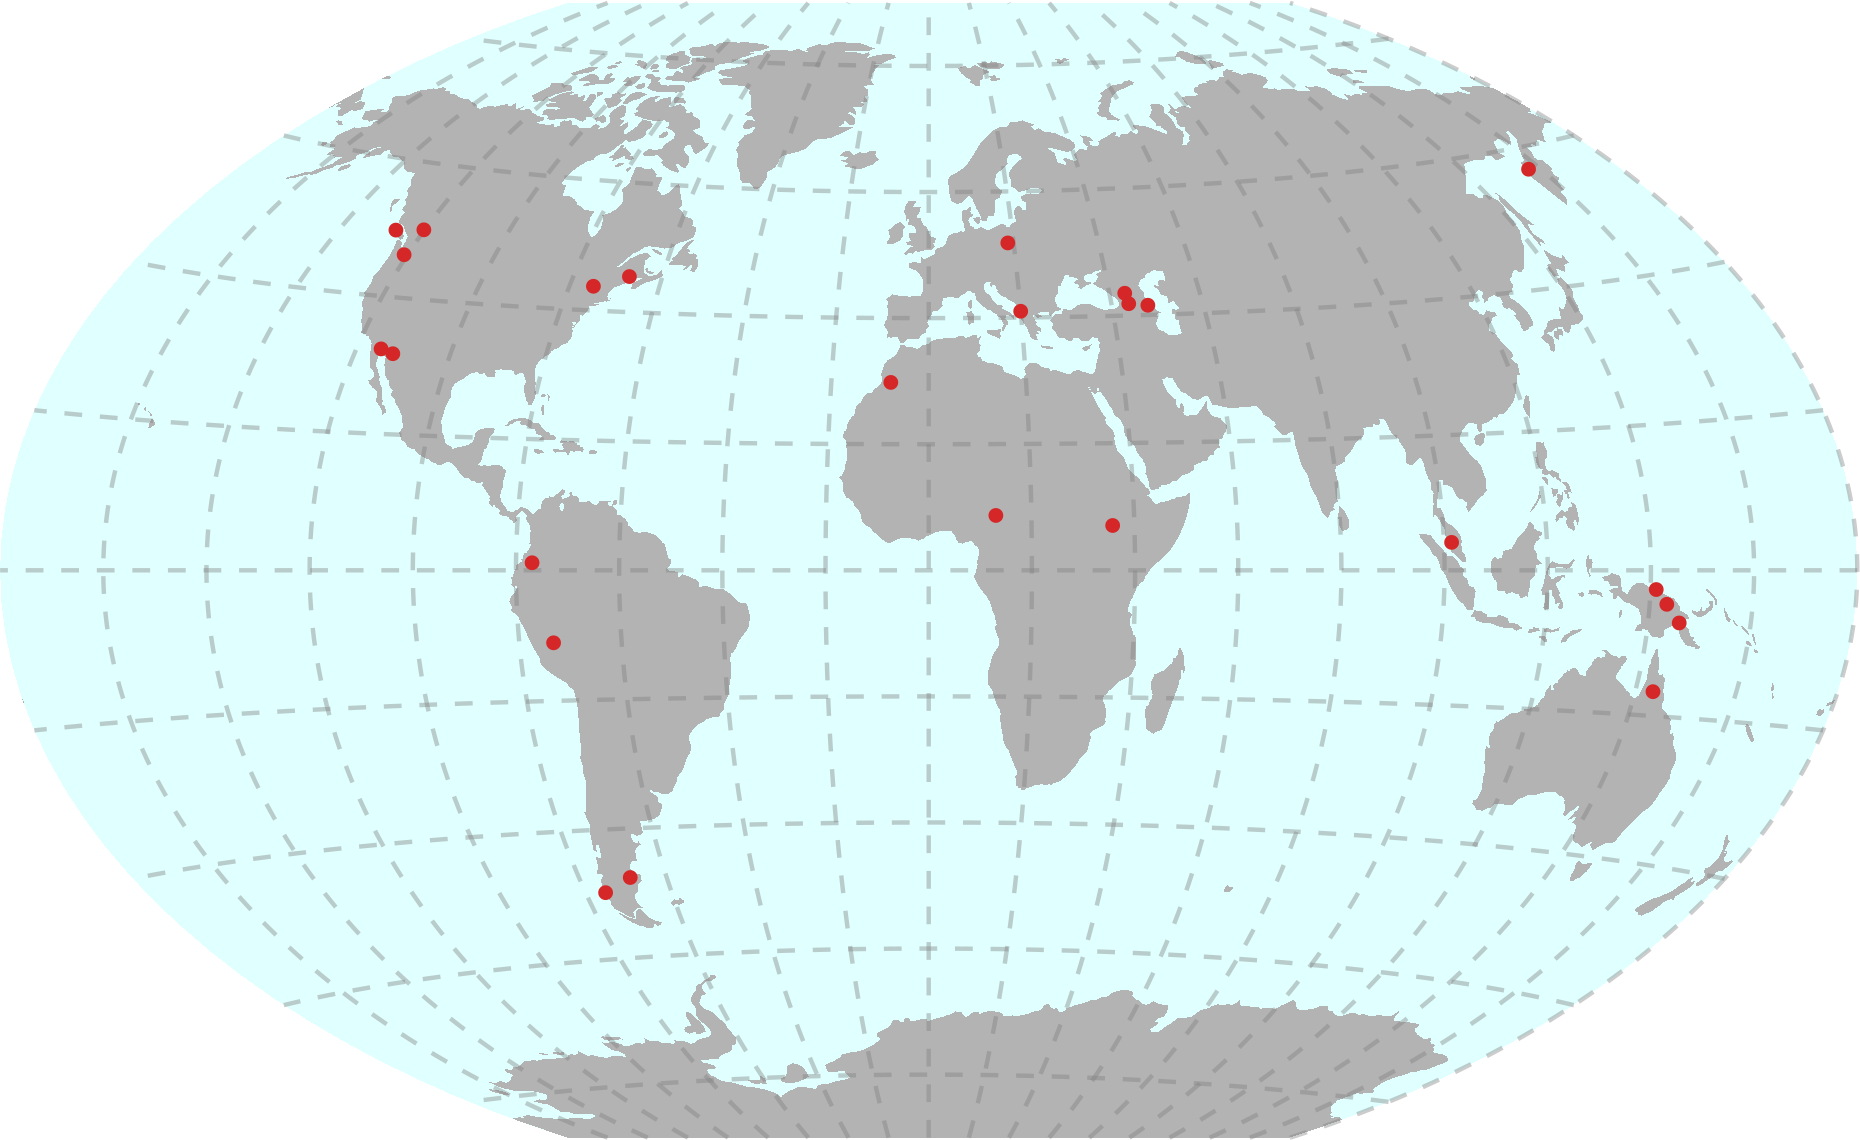
\includegraphics[width=\textwidth]{figures/fig81.png}
\caption{\label{fig:8.1}Geographical distribution of languages in Highly Complex portion of sample.}
\end{figure}

  In \figref{fig:8.1}, there are the expected clusters of languages in the Pacific Northwest and Caucasus regions. Smaller clusters of unrelated languages include: Tohono O’odham and Cocopa in the Sonoran Desert region, Passamaquoddy-Maliseet and Mohawk in the northeastern region of the USA and Canada, and Qawasqar and Tehuelche in Patagonia. Even three of the languages with Highly Complex syllable structure as a minor pattern -- Alamblak, Menya, and Wutung -- are found in relative geographic proximity to one another in New Guinea. In most of these regions, there is historical and linguistic evidence of long-term cultural contact among unrelated ethnolinguistic groups. For example, while Tohono O’odham and Cocopa are not known to have been in intensive direct contact with each other, recall the discussion from \sectref{sec:8.4.3} noting that languages from the Tepiman branch of Uto-Aztecan and those of the Yuman family are known to have a long history of contact. 

  In a few cases, the evidence suggests that phonological patterns of languages in the sample have changed in the context of language contact. As mentioned in \sectref{sec:8.4.3}, Lelepa is known to be in direct contact with other languages with similarly complex syllable patterns. In the preface to a volume titled \textit{Angan Languages Are Different}, \citet[4]{Healey1981} writes that the Angan language family to which Menya belongs is “characterized by phonological complexity unusual in this country”. Wurm and colleagues remark on the “aberrant” nature of Angan languages within the Trans-New Guinea context and suggest that the characteristics of this small family suggest a “strong super-imposition upon an older, probably unrelated language type” (\citeyear{WurmEtAl1977}: 310). This seems to imply a contact or substrate origin for some of the phonological differences that Angan languages exhibit.

  That syllable structure complexity has been described as a feature of linguistic areas known for their diversity such as the Pacific Northwest and the Caucasus suggests that such patterns can spread from one language to another in situations of heavy language contact and bi- or multilingualism. Yet we know from observations of loanword adaptation that novel syllable structures are not easily borrowed; one of the major crosslinguistic loci of epenthesis processes is precisely in this context \citep{Hall2011}. This raises the question of how syllable patterns, especially highly complex ones that are crosslinguistically rare to begin with, converge in languages in situations of contact.

  It has been noted that in situations of language contact, prosodic and suprasegmental phenomena are more likely to diffuse than phonemes (chapters in \citealt{AikhenvaldDixon2001b}). There is a growing body of empirical evidence for this observation. \citet{Mennen2004} found that Dutch-Greek bilinguals who acquired Greek in adulthood transferred peak alignment patterns from Dutch into their Greek speech. Native speakers of Tswana were found not to apply phrase-final lengthening in their English speech, in accordance with their L1 patterns, setting the intonational properties of their speech apart from those of South African English and Afrikaans English speakers (\citealt{CoetzeeWissing2007}). \citet{Simonet2011} reports that Spanish-Majorcan Catalan bilinguals tend to transfer utterance-final pitch accents from their L1 to their L2. In a study of English-Mexican Spanish bilinguals in Los Angeles, \citet{Robles-Puente2014} found that both speakers who had moved to Los Angeles in childhood and those who had been born in Los Angeles to immigrant parents retained Mexican Spanish intonational contours in their Spanish and English speech.

  As discussed in previous chapters, the component of speech prosody which has been most often associated with syllable complexity is speech rhythm. Instrumental investigations providing evidence for the influence of L1 rhythmic patterns on L2 (and sometimes vice versa) are becoming more prevalent in the literature. \citet{WhiteMattys2007} measured acoustic correlates of rhythm in native and non-native English, Dutch, Spanish, and French speech. They found that L1 has an effect on L2 which is observable in the rhythm metrics VarcoV (standard deviation of vocalic interval duration divided by the mean vocalic duration) and \%V (proportion of vocalic intervals). In L2 speech, the values for these metrics usually fell somewhere between the values measured for native speech in each of the languages. A comparison of the Pairwise Variability Index (PVI) metric in the speech of Spanish monolinguals and speakers of Hispanic English revealed a Spanish substrate influence on the speech of the latter \citep{Carter2005}. Further, the rhythmic properties of Hispanic English were found to be quite uniform across speakers regardless of generation, which the author suggests may be indicative of long-term persistence of  the substrate influence. \citet{Robles-Puente2014} found that English-Spanish bilinguals who had been in Los Angeles since childhood or were raised there by immigrant parents showed Spanish-like rhythm in both languages. Finally, the effect may go the other way as well: Afrikaans-Spanish bilinguals who had been living in a Spanish-dominant environment (in Patagonia) for at least two-thirds of their lives were found to show more Spanish-like values for the nPVI-V metric in their Afrikaans speech than non-bilingual Afrikaans speakers \citep{CoetzeeEtAl2015}. 

  Because the rhythm metrics mentioned in the research above correspond to durational properties of consonant and vowel intervals, they may reflect timing patterns which relate directly to syllable structure complexity. There is at least one case in which the instrumentally-confirmed rhythmic properties of a language correspond to a historically documented process of contact-induced syllable structure change. This is the case of Moroccan Arabic.

  Dialects of Arabic spoken in North Africa, also known as Western Arabic, have often been said to have phonetic and rhythmic properties which differ markedly from those of the dialects spoken in the Middle East (Eastern Arabic dialects). In a perceptual experiment, native speakers of various dialects of Arabic were able to correctly identify Arabic speakers as coming from North Africa or the Middle East 98\% of the time \citep{BarkatEtAl1999}. In this task, speakers mentioned that the perceptual characteristics of Western Arabic which helped them make this identification were that it sounded “faster” than Eastern Arabic and had a “jerky” or “halting” sound \citep{GhazaliEtAl2002}. All varieties of Arabic have been described as stress-timed in the literature; however, the salient perceptual differences between Western and Eastern Arabic have prompted instrumental investigations into the nature of rhythmic timing in the various dialects. An analysis of the acoustic properties of Western (specifically Moroccan, Algerian, and Tunisian) and Eastern (specifically Egyptian, Jordanian, and Syrian) dialects of Arabic revealed extreme differences in their values for metrics used to quantify speech rhythm properties \citep{HamdiEtAl2004}. Western Arabic dialects had values for ΔC (standard deviation in consonant intervals) and \%V (proportion of vocalic intervals) which were even more extreme than those found for the ‘prototypical’ stress-timed language English. The ΔC and \%V values for Eastern Arabic dialects put these languages closer to French, which is said to have syllable timing. Of the three Western Arabic dialects, Moroccan Arabic had the most extreme high ΔC and low \%V values. The authors attributed this pattern to the frequent deletion of short vowels in this dialect, which creates consonant clusters and syllabic consonants, and also to the generally shorter duration noted for both phonologically long and short vowels in this dialect as compared to Eastern Arabic dialects.

  \citet{Chtatou1997} notes that the phonetics, phonology, morphology, and lexicon of Moroccan Arabic have been heavily influenced by contact with the Amazigh (Berber) languages indigenous to the region, including Tamazight, Tarifit, and Tashlhiyt, with influences being likened to heavy substrate effects. In the most recently Arabized regions, Moroccan Arabic may be so phonetically different from other Western dialects of Arabic that speakers of the other dialects have trouble understanding it (ibid. 105). Some of the phonetic differences can be attributed to patterns of vowel reduction resulting in complex consonant clusters. Recall from previous examples that Tashlhiyt has highly complex syllable structure due to the prevalence of syllabic consonants in the language, which frequently result in long word-marginal strings of consonants or even words without vowels. In accordance with the phonetic patterns of local Amazigh dialects, Moroccan Arabic varieties are characterized by rampant vowel reduction resulting in tautosyllabic clusters or syllabic consonants, depending on the analysis. This is apparent when comparing Classical Arabic (CA) forms to their Moroccan Arabic (MA) equivalents: e.g., CA /na.di.ma/ > MA /n.dm/ ‘to regret;’ CA /ta.qaː.ba.la/ > MA /t.qaː.bl/ ‘to meet’ \citep[110]{Chtatou1997}. We see from comparison with Eastern dialects of Arabic that this pattern is unique to Moroccan Arabic. Other dialects have kept most of the vowels of Classical Arabic, though vowel quality changes may have occurred \REF{ex:8.5}:

\ea\label{ex:8.5}
  Comparison of forms in Classical Arabic, Eastern dialects, and Moroccan Arabic

  CA \textit{katabtu} > Egyptian Arabic \textit{katabt} > MA \textit{ktbt} ‘I wrote’ 

  CA \textit{taktubu} > Saudi Arabic \textit{tiktib} > MA \textit{ka tktb} ‘you (\textsc{m}) write’

  CA \textit{taskunu} > Iraqi Arabic \textit{tiskin} > MA \textit{ka tskn} ‘you (\textsc{m}) live’
\citep[111-12]{Chtatou1997}
\z

This pattern of vowel deletion is extremely productive and applied quite generally to loanwords. The most common pattern in syllable structure adaptation in lexical items from Classical Arabic is the deletion of short vowels and the preservation of long ones, as in the word for ‘to meet’ given above. Similar patterns may be observed in the adaptation of French loanwords into Moroccan Arabic: e.g., Fr. \textit{direction} > MA \textit{drksjuːn} ‘direction;’ Fr. \textit{tracteur} > MA \textit{trktu}ː\textit{r} ‘tractor’ (\citealt[116]{Chtatou1997}; note that the final prosodically prominent vowel has been retained). \citet{Sayahi2005} describes a number of patterns by which vowel-initial Spanish loanwords into Moroccan Arabic are made to have more complex syllable structure: e.g., Sp. \textit{equipo} > MA \textit{lkipo} ‘team;’ Sp. \textit{espia} > MA \textit{spia} ‘spy;’ Sp. \textit{enfermero} > MA \textit{frmiro} ‘nurse.’

  The phenomenon described above is quite interesting, because reported instances of nativization of syllable patterns in the literature tend to involve the simplification of patterns; e.g. English \textit{technostress} > Japanese \textit{tekunosutoresu} \citep[69]{Kay1995}. Similarly, when languages with complex syllable structure borrow words from languages with simpler syllable structure, segmental patterns are often nativized, but syllable patterns are usually retained; e.g. Japanese \textit{tsunami} [t͡sɯnami] > English [su]\textit{nami}; English \textit{Hamlet} > Russian [ɡ]\textit{am}[lʲ]\textit{et}. Both Moroccan Arabic and Amazigh varieties have phonological words which are similar in shape to the Classical Arabic, French, and Spanish source words given above; e.g., Tashlhiyt \textit{tifunasin} ‘cows,’ Moroccan Arabic \textit{hadak} ‘\textsc{dem.}’ Thus it is not readily apparent why loanwords would be borrowed in such a way as to create such complex onsets. This is a case in which morphosyntactic patterns of the language may have some effect on the phonological adaptation of loanwords. In Moroccan Arabic, as in Tashlhiyt, the inflectional morphology of the language relies in part on nonconcatenative processes which can be lexically determined and dependent upon the phonological form of words, many of which have complex clusters and also tend to be monosyllabic \citep{Heath2007}. Perhaps loanword adaptation is in part affected by analogy to such patterns. Nevertheless, as we know from the historical and comparative evidence, those very patterns originated in highly productive patterns of vowel reduction which were carried over from Amazigh.

  The case of Moroccan Arabic suggests that native properties of speech rhythm, including vowel reduction and tendencies toward longer consonant intervals and shorter vowel intervals in speech, may be transferred by speakers to an L2 much in the same way that intonational contours are transferred. In situations of intense cultural contact and high rates of bilingualism and multilingualism, it is easy to imagine rhythmic properties being transferred in this way among unrelated languages with the effect that similar syllable patterns may be found in them.

\subsection{Development of Highly Complex syllable structure: Conclusions and questions}\label{sec:8.4.6}

  Syllable structure has long been known to become more complex through processes of vowel reduction. The associations between syllable complexity and other phonetic, phonological, and morphological properties suggest that the path to highly complex syllable structure additionally tends to include other specific processes and properties in addition to vowel reduction or deletion.

  It is clear from the crosslinguistic trends, the comparison of related pairs of languages, and the case study of Lezgian that stress-conditioned vowel reduction, in particular, is almost always relevant in the development of highly complex syllable structure. The findings here also point to the persistence and increasing prevalence of vowel reduction as syllable structure becomes more complex. Morphologically complex contexts are more often than not a factor, though the Lezgian example shows that this does not always have to be the case.

  Consonant inventory size is additionally strongly associated with syllable complexity, and specific consonantal articulations with either end of the syllable complexity scale. However, the crosslinguistic patterns in specific segmental contrasts were not strongly upheld in the comparisons of related languages. The comparisons of related pairs of languages largely showed the expected patterns with respect to a higher prevalence of consonant allophony in the languages with simpler syllable patterns, but in the Lezgian example, place assimilation of consonants to vowels occurs concurrently with, or shortly following, vowel reduction. Perhaps the inconsistent patterns with respect to consonantal articulations and consonant-affecting processes are related to the speed with which vowel reduction affects syllable structure patterns, or even the specific kind of vowel reduction operating within a language (e.g., quality, devoicing, reduction in duration). That is, the same underlying mechanisms for vowel reduction may also condition consonant processes that lead to larger inventories, albeit in complex and varied ways. Without detailed historical accounts, it is difficult to identify the specific patterns that consonant changes may take as part of a larger process of syllable structure change. However, the consistent differences in consonant phoneme inventory size in languages with simpler and more complex syllable structure suggest that there is a non-coincidental relationship there.

  Another important consideration in the development of highly complex syllable structure is the issue of contact and transfer of rhythmic properties from one language to another. It is not clear whether we should expect many correlates of highly complex syllable structure to occur when syllable complexity is increased as a result of rhythmic transfer from one language to another in situations of intense contact. Perhaps this is another case where segmental, allophonic, and even morphological patterns may deviate from the predictions derived from the crosslinguistic patterns.

  A question that still remains open is how, specifically, the diachronic path leading to highly complex syllable structure gets started in a language. In light of the findings and discussions above, I have one specific hypothesis which is based on observations of vowel reduction patterns in languages with Simple syllable structure. Recall from the summary of vowel reduction processes in \sectref{sec:6.3.6} that the most common process type in the Simple category is the devoicing of vowels at word or phrase/utterance margins. In the comparison of pairs in \sectref{sec:8.4.3}, 3/4 languages with the simpler syllable patterns (Ute, Apurinã, and Maori) have vowel devoicing as an outcome of vowel reduction. This proportion, though derived from a tiny group of languages, is larger than the overall proportion of languages in the Simple category which have devoicing as an outcome of vowel reduction (6/13). That is, in language families in which both extreme syllable patterns occur, such that there is the phonological and morphological potential for languages with simpler syllable patterns to follow a similar path as their relatives with more complex phonotactics, devoicing is very likely to be an outcome of vowel reduction in the languages with simpler patterns. This is interesting, because vowel reduction resulting in devoicing may be a more likely source of incipient syllable structure change than other forms of reduction. This is because devoiced vowels, especially in domain-marginal contexts, may be easily lost or restructured as glottal fricatives or aspiration. In Apurinã, it has been noted that stops become aspirated preceding a devoiced unstressed vowel \REF{ex:8.6}.

\ea\label{ex:8.6}
  \etriple{Apurinã}{Arawakan}{Brazil}

/kaˈjati/

[kaˈjatʰi̥]\\
\glt ‘paca (large rodent)’
\citep[60-1]{Facundes2000} 
\z

  The Apurinã example suggests that the properties of the devoiced vowel are becoming associated with the consonant, providing an ideal context for sound change, and in this case, syllable structure change.\footnote{{On the other hand, the aspiration analysis may simply be another way of noting the devoiced vowel.}} As described in \sectref{sec:3.2.3}, a similar process of vowel devoicing in Ute has already affected the syllable patterns in that language. If domain-marginal vowel devoicing occurs in a language with word stress, perhaps such devoicing processes could disrupt the rhythmic patterns of the language, leading eventually to a stronger role of stress and associated segmental effects. This topic would be a good avenue for further research.

  In \figref{fig:8.2} I show how highly complex syllable structure and its associated properties might develop out of simpler syllable structure and its properties, according to the findings here.

\begin{figure}
\begin{tikzpicture}[>=Triangle,baseline]
\graph [branch down=7\baselineskip,grow right sep=1cm,nodes={font=\small,draw,rounded corners=2pt,text width=2.25cm,align=left}] {
a[as={stress-conditioned allophonic C processes}] -> {b[as={phonologiza\-tion of fortition, assimilation processes}] -> d[as={palato-alveolar, uvular, affricate, ejective phonemes}], c[xshift=-1.625cm,as={phonologiza\-tion of lenition processes, phonemicization of associated articulations}]};
e[as={domain-conditioned V devoicing},text width=2cm] ->[dashed] f[as={\itshape destabilization of stress patterns?},draw=none,text width=2.1cm] ->[dashed] {g[as={stress-conditioned V reduction, deletion},text width=2cm],h[as={syllabic Cs},yshift=3\baselineskip]} -> i[as={increased V reduction},text width=2cm] <- j[xshift=-3.25cm,yshift=-7\baselineskip,draw=none,as={\itshape stronger effects when morpheme/word ratio high, grammatical morphemes involved?},text width=2cm];
};
\draw[thick,-{Triangle[]}] (current bounding box.north west) ++(0,\baselineskip) -- (current bounding box.north east) node[above,at start,anchor=south west] {Simple} node[above,at end,anchor=south east] {Highly Complex};
\end{tikzpicture}
\caption{\label{fig:8.2}Proposed path of development for highly complex syllable structure out of simpler syllable patterns.}
\end{figure}


  In the discussions above I explored how highly complex syllable structure might arise over time in special phonological, morphological, and even sociolinguistic contexts. While there are still open questions regarding the details of these paths, I believe that the evidence shows that the processes involved are quite natural and common patterns of language change, a fact that stands in stark contrast to the frequent description of highly complex structures as marked or dispreferred. In the following section I discuss the long-term stability of these structures.

\section{Highly complex syllable structure: A stable and motivated pattern}\label{sec:8.5}

  Recall from the discussion of the literature in \chapref{sec:1} that many of the properties of highly complex syllable structure -- the size and composition of clusters, the presence of syllabic obstruents, its association with morphological complexity -- are crosslinguistically rare and/or theoretically problematic. Abstract theoretical accounts for the structures rarely touch upon practical aspects of these ‘dispreferred’ patterns such as their maintenance and stability in speech communities in the long term. I discuss some of these issues here.

\subsection{Synchronic stability of Highly Complex syllable structure}\label{sec:8.5.1}

  In \chapref{sec:6} it was found that 21/25 of the languages in the Highly Complex category were reported to have processes of vowel reduction. The 15 languages in this category with stress-conditioned vowel reduction had on average three such processes as ongoing synchronic patterns. Altogether, processes of vowel deletion or reduction were found to alter syllable patterns in 13 of the languages in this category, either by turning onsets into codas, producing tautosyllabic clusters, or producing syllabic consonants. As mentioned in that chapter, what the crosslinguistic data suggests is that vowel reduction has the strongest effects on syllable structure in languages in which such processes have previously altered the canonical syllable patterns.

  Because highly complex syllable patterns are so crosslinguistically rare and ‘dispreferred,’ we might expect to see in these languages more instances of simplification of syllable patterns than instances of syllable structure becoming more complex. As the discussion of directionality in \sectref{sec:8.4.1} suggests, this does not seem to be the case. In that discussion, I mentioned incipient processes of variable epenthesis and historical processes of cluster simplification. Here I present additional information regarding the stability of highly complex syllable structure by discussing regular (phonologized) processes of epenthesis and active processes of cluster simplification.

  An analysis of the languages in the Highly Complex category revealed that nine languages have regular phonological processes of epenthesis which break up consonant clusters. There are two kinds of epenthesis patterns which are characteristic of the languages of this group: processes which break up sequences of sounds which are identical or highly similar (e.g., sequences of sibilants), and processes which break up sequences of two sonorants or a sonorant and obstruent. I give an example of the latter process type in \REF{ex:8.7}.

\ea\label{ex:8.7}
  \etriple{Yakima Sahaptin}{Sahaptian}{USA}

\ea  /ʔínm/\\\relax
  [ʔínɨm]\\
  \glt ‘excessively’

\ex  /t͡ɬ’jálm/\\\relax
  [t͡ɬ’jálɨm]\\
  \glt ‘Cle Elum (place name)’

\ex  /talújm/\\\relax
  [talújɨm]\\
  \glt ‘nail’
\z
(\citealt[28]{HargusBeavert2006})
\z

Similar processes can also be found in Kabardian and Doyayo, among others. What is interesting about such patterns is that they do not target the long sequences of obstruents which are prototypical of highly complex syllable structure.

  An analysis of active (variable) processes of consonant deletion resulting in cluster simplification turned up similar results. There are ten languages with such patterns. Interestingly, such processes typically affect sonorants or glottal fricatives in these languages. While the affected sound in the example in \REF{ex:8.8} is transcribed as a voiced fricative, it patterns phonotactically with sonorants in Georgian (\citealt{ShostedChikovani2006}: 261).

\ea\label{ex:8.8}
  \etriple{Georgian}{Kartvelian}{Georgia}

/vpɾt͡skʰvni/

[ɸpɾt͡skʰvni] {\textasciitilde} [pɾt͡skʰvni]\\
\glt ‘I peel’

(\citealt{ShostedChikovani2006}: 261)\footnote{{Elsewhere in this book I have followed \citet{Aronson1991} in transcribing the voiced labial fricative of Georgian as bilabial /β/; however, some researchers classify it as a labiodental /v/. I use /v/ in this example to preserve Shosted \& Chikovani’s transcription.}}
\z

Again, the prototypical syllable patterns of these languages are not strongly affected by such processes. It should also be noted that four of the languages with processes like these have Highly Complex structures as a minor pattern (Alamblak, Kunjen, Menya, and Wutung).

  The distribution of processes of epenthesis and consonant deletion, as compared to the distribution of vowel reduction processes, suggests that despite theoretical issues of analysis, highly complex syllable structure is neither problematic for speakers, nor synchronically unstable in speech communities. The phonetic processes responsible for creating these syllable patterns appear to be both remarkably persistent and more prevalent than processes which ‘repair’ them, at least in languages which have Highly Complex syllable structure as a prevalent pattern.

\subsection{Diachronic stability of syllable complexity}\label{sec:8.5.2}

  Complex syllable structure may show long-term stability within language families and regions. This is apparent in examining the geographical distribution of maximal syllable structure patterns. In constructing the language sample for the current study, it was impossible to find the Simple pattern within Eurasia, and very difficult to find such patterns in North America, such that 2/3 languages from this region in the Simple portion of the sample actually have Moderately Complex patterns. If we assume that the complex syllable patterns of these regions developed at some point out of simpler patterns, then the geographical distributions suggest that, once it develops, syllable complexity tends to persist for long periods of time. Similarly, a recent study of maximal syllable shapes in four proposed linguistic areas found that the patterns were more closely associated with language families than with regions, though there was limited evidence for convergence in parts of the Caucasus and Pacific Northwest (\citealt{NapoleãodeSouza2017}). The author’s interpretation of the findings was that syllable structure patterns may be a generally stable phonological property of languages, persisting for long periods of time within language families. If one considers only the universal preference for CV structures, these distributional facts are unexpected. We might expect that strong cognitive or physiological pressures favoring CV over all other syllable types would manifest crosslinguistically in such a way that languages with canonical (C)V patterns could be found in any language family or region.

  From a diachronic point of view, the observed patterns may relate to the way that vowel reduction, vowel epenthesis, and consonant deletion tend to operate within languages. Vowel deletion may cause canonical syllable patterns to change from fairly simple to quite complex in a relatively short period of time, such that a language which previously had only simple onsets may, just a few generations later, have a wide variety of highly complex clusters (e.g., Lezgian). The opposite scenario, in which highly complex syllable patterns in a language are uniformly simplified by epenthesis in a short period of time, seems very unlikely. Crosslinguistically, epenthesis processes tend to target specific phonotactic environments or sequences of sounds \citep{Hall2011}. While such processes might simplify some specific syllable shapes in a language, they might leave many others unaffected, such that the overall syllable pattern of the language is still complex (cf. the Yakima Sahaptin example in 8.7). Unless vowel epenthesis becomes a completely general process, or occurs in multiple iterations with different consonant sequences (both of which seem unlikely given crosslinguistic patterns), it is hard to imagine such a process dramatically changing the syllable patterns of a language in a short period of time. This also seems unlikely from an articulatory point of view, given that the widespread temporal adjustments to gestural organization required of such a scenario would run against general tendencies towards increased overlap and reduction of gestures (\citealt{BrowmanGoldstein1992b}). Similarly, processes of cluster reduction, as noted above, often target specific sequences, and it is hard to imagine these operating so generally as to obliterate both word-marginal and word-internal clusters in a language to the point where they dramatically affect canonical syllable patterns. 

  It seems that in the case of syllable structure, a high degree of complexity may be introduced quite rapidly into the system, but once there, it is difficult to completely remove. Historical processes suggest this is the case. In the Middle English (ME) period, a series of vowel epenthesis processes targeted certain consonant sequences in the language which had been present in Old English (OE): e.g., OE \textit{niht} > ME \textit{nyhyt} ‘night;’ OE \textit{myln} > ME \textit{milne} ‘mill’ (\citealt{Jones1989}: 167, 170). Similarly, some codas were lost through sonorization processes: e.g., West Saxon OE \textit{he\={} ɡ} > ME \textit{hei} ‘hay’ (ibid. 150). Meanwhile, cluster simplification processes reduced /kn/ and /gn/ onsets \citep{Minkova2003}. Despite these changes to syllable patterns, which were quite widespread judging from orthographic evidence, onset clusters such as /pl/ and /fr/, and codas such as /nd/, were not affected by such processes: cf. OE \textit{ploga} ‘plough,’ OE \textit{fre}\textsf{\={} }\textit{ond} ‘friend.’ Thus while syllable complexity was simplified at the level of specific sequences in the language, and simple syllable shapes perhaps became more frequent, the canonical syllable patterns of the language were not strongly affected. By comparison, later processes of vowel deletion added considerably to the complexity of coda patterns in the language, yielding what are today the maximal tautosyllabic clusters in the language: \textit{si}[ksθs], \textit{te}[ksts], and so on.

\subsection{Phonetic properties of Highly Complex syllable patterns and long-term stability}\label{sec:8.5.3}

  Researchers often remark upon the salient phonetic characteristics of highly complex syllable patterns. In \sectref{sec:3.4.3} I presented a variety of phonetic descriptions of consonant (usually obstruent) clusters in languages from the Highly Complex portion of the sample. The accounts describe the clusters in these languages as being characterized by ‘open transition,’ ‘transitional vocoids,’ ‘overtones,’ ‘strong aspirated release,’ ‘audible intervals,’ and so on. These phonetic properties are described for sequences analyzed as clusters and those analyzed as syllabic obstruents, and all share properties typical of intrusive vowels as defined by \citet{Hall2006}. In my previous discussion of these patterns, I concluded that such transitions are a prominent characteristic of Highly Complex syllable structure and constitute a phonetic correlate of this language type. I propose that these salient phonetic characteristics, which derive from temporal properties of gestural organization, facilitate the long-term maintenance and stability of highly complex syllable patterns which most models of the syllable predict to be dispreferred.

  There is a small body of research which relates the temporal properties of gestural organization of obstruent sequences to perceptual recoverability. Consonant clusters have been found to be characterized by less overlap between gestures when occurring in word-initial position than in other positions (cf. \citealt{Byrd1996a} for English). In a perceptual recoverability account, word-initial position may correspond to utterance-initial position in discourse. If a word-initial sequence of obstruents, especially stops, occurs in utterance-initial position, there is no vowel preceding the first consonant which could provide acoustic cues as to its place of articulation. A release of the first stop would cue acoustic information on its place of articulation, while heavy overlap with the following consonant would obscure such acoustic cues. Perception of the first stop would be additionally facilitated if a vocalic transition is present, since this allows for a greater distribution of acoustic cues in time (\citealt{RidouaneFougeron2011}: 294). In this view, gestural organization strategies resulting in a temporal lag between word-initial obstruents may have a perceptual motivation; that is, overlap between consonant gestures may be suppressed in order to preserve phonetic cues.

  Perceptual recoverability has been suggested as a motivation behind timing patterns observed in clusters in Korean (\citealt{SilvermanJun1994}), Tsou \citep{Wright1996}, Georgian \citep{ChitoranEtAl2002}, and Tashlhiyt (\citealt{RidouaneFougeron2011}). Some of these studies have shown that it is not just word onset position, but also the relative place of articulation of the consonants in sequence which contribute to observed temporal lag, which somewhat weakens the original argument for perceptual recoverability. Indeed, most of the phonetic descriptions of highly complex clusters in \sectref{sec:3.4.3} do not refer specifically to word-initial or even onset environments, but instead mention specific sequences of consonants. In Cocopa, for example, transitional elements can be found in at least some word-final consonant sequences \REF{ex:8.9}.

\ea\label{ex:8.9}
  \etriple{Cocopa}{Cochimi-Yuman}{USA}

k\textsuperscript{a}myu\'{} x\textsuperscript{i}ɬʲ\\
\glt ‘I hope that somehow you will’
\citep[47]{Crawford1966}
\z

Additionally, \citet{ChitoranCohn2009} note that in Georgian onsets, the timing lag between consonant gestures is larger than what is needed for the release burst to be perceptually recoverable. They further suggest that timing differences between consonant sequences in Georgian reflect phonologized patterns of language-specific gestural organization.

  Considering that obstruent clusters in languages with highly complex syllable structure come about through vowel reduction, and that place characteristics of the original vowel may be retained in release bursts (cf. descriptions of clusters in Lezgian and Tohono O’odham in \sectref{sec:3.4.3}), it seems more likely that perceptual recoverability is an effect of, rather than a motivation for, the gestural organization of clusters in these languages. I suggest that the gestural timing and perceptual properties of such sequences may facilitate the long-term maintenance of highly complex syllable patterns by making them less susceptible to complete overlap resulting in consonant deletion (\citealt{BrowmanGoldstein1990}).

\section{Topics for further research}\label{sec:8.6}

  In this book I have shown that highly complex syllable structure is a holistic linguistic type associated with a number of phonetic, phonological, and morphological correlates. Additionally, the crosslinguistic patterns identified here may point to general tendencies in the diachronic development of these structures. However, there are many ways in which the studies here can be expanded. Some of the results also suggest lines of research outside of the range of standard phonological typology.

  An issue which should be explored in more depth is that of the type frequency of syllable patterns. This issue was touched upon only briefly in the discussion of the prevalence of highly complex patterns in \chapref{sec:3}. A finer-grained analysis of frequency patterns may refine our understanding of how processes of vowel reduction and consonant allophony work their way through the language as syllable structure changes. Similarly, the treatment of morphology was necessarily brief and general in the current study, but there is ample ground for further research here. Relevant topics may include the type (e.g., prefixing, suffixing, infixing, templatic, etc.) and function (inflection, compounding, lexical class-changing derivation, lexical affixation, etc.) of morphological patterns which occur in tautosyllabic clusters of different degrees of complexity. Additionally, it would be interesting to establish a crosslinguistic range for the distribution of morphologically simple and complex tautosyllabic clusters or syllable inventories, as the results here point to a great deal of variation with respect to such distributions even within the Highly Complex portion of the sample. Though such studies have been conducted for a handful of European languages (\citealt{DresslerDziubalska-Kołaczyk2006}, \citealt{DresslerEtAl2010}, inter alia), a truly global examination of these issues could better inform our understanding of the development of phonotactic complexity. A preliminary investigation in this vein suggests that at least for onsets, morphologically complex consonant clusters are more restricted in their structure and distribution than morpheme-internal clusters in a variety of ways \citep{Easterday2019}.

  Another issue which deserves more attention is that of language contact and syllable structure complexity. While linguistic areas such as the Pacific Northwest and the Caucasus region are well known for unusual syllable complexity, possibly as an effect of contact, some patterns noted above suggest that this phenomenon may be relatively frequent at an even smaller scale. The situation of Lelepa and its neighbors is especially striking because it shows emerging complexity at a very local level in a situation of contact, but within a larger family which is famous for its simple syllable patterns (Oceanic). A global survey of similar small-scale clusters of syllable patterns may reveal important information about the role of contact in the development of phonological complexity.

  Finally, the results of the current study suggest that there are properties of gestural organization associated with both synchronic characteristics of highly complex syllable patterns and diachronic stages of their development. Synchronically, the obstruent clusters associated with these syllable patterns are characterized by open transitions between consonantal gestures which may in many cases have their source in processes of vowel reduction. Diachronically, the contrastive consonant articulations associated with these languages may originate in patterns of increased overlap of consonantal and vocalic gestures and strengthening of consonantal gestures at some point in the history of these languages, perhaps even before the development of complex syllable patterns. There is a growing literature of instrumental investigations of gestural organization in the syllable patterns of diverse languages. Many of these studies are relevant to the issues examined here concerning properties of consonant clusters (cf. \citealt{GoldsteinEtAl2007} for Georgian and Tashlhiyt, \citealt{HermesEtAl2013} for Italian, \citealt{Marin2014} for Romanian, \citealt{Butler2015} for Khmer and Bunong, \citealt{MarinEtAl2017} for seven European languages) and syllabic consonants (cf. \citealt{HermesEtAl2011} for Tashlhiyt, \citealt{PouplierBeňuš2011} for Slovak). The findings in the current study reveal a prevalence of vowel reduction in languages with more complex syllable patterns and suggest a prevalence of coarticulation of consonants with adjacent vowels and strengthening in languages with simpler syllable patterns. In light of these findings, it would be interesting to instrumentally investigate general patterns of gestural organization as they pertain to those specific issues in languages with differing syllable complexity.
